\section{Optimal Fine-gained Pruning}\label{sec:pruning}



In this section, we present our final contribution: a novel, fine-grained pruning stage that significantly enhances the performance of hierarchical kNN join indexes. This technique acts as a crucial intermediate filter, performing point-wise pruning in a low-dimensional space to bridge the gap between coarse-grained cluster-level pruning and expensive full-dimensional verification. Although this method is generally applicable to any index following a progressive granularity strategy, we focus here on its integration into our \dualtree\ framework to optimize \fdknnj. More importantly, we develop a rigorous theoretical model to derive the \textbf{optimal projection dimensionality} for this stage, maximizing its efficiency by formally balancing pruning power against computational overhead.

\subsection{Insufficient pruning at the non-leafnodes on \dualtree}
\begin{comment}
While the original kNN Search and RkNN Search algorithm on \hdrtree and \deltatree directly apply full-dimensional distance computation at the leafnodes to finally identify the kNN or RkNN members of the query points, pruning strategy based on low-dimensional point-to-point distance computation still remains effective at leafnodes. This is due to the fact that, when the search progresses to the leaf nodes, there are still many data points far from the query point that have not been pruned and thus remain. 

This is because pruning at the non-leafnodes of the \dualtree is insufficient, tending to  incorrectly retain points that should be excluded, a phenomenon known as false positives.

The reason of insufficient pruning is resulted from the cluster-level pruning at the non-leafnodes, in the process of which, data points are pruned or reserved cluster wise based on the condition $dist_{PC}(center(C_j), u)-radius_{PC}(C_j)<dist\_prune$ (used in the \deltatree part) or the condition $dist_{PC}(center(C_j), q) - radius_{PC}(C_j) < dist_\text{MkNN}(C_j)$ (used in the \hdrtree part). 

If the inequality above holds, implying that the visited cluster is determined to be retained, there is still a possibility that the data points within the cluster are far from the query point and can therefore be pruned. This occurs when the data point providing $radius_{PC}(C_j)$ in the cluster is located on the far side of the query point. Two examples are presented below in Figure \ref{fig:knn_error} and Figure \ref{fig:rknn_error}. 





\begin{example}[False positive error in kNN Search]
In Figure \ref{fig:knn_error} where a cluster $C_j$ at a non-leafnode in the \deltatree part of a \dualtree structure is visited in the kNN Search process of a query point $u_q$, the condition $dist_{PC}(center(C_j), u)-radius_{PC}(C_j)<dist\_prune$ holds but it is obvious that no data points in $C_j$ should be retained because all of their distances to $u_q$ exceed $dist_{prune}$.  
\label{example:false positive error in kNN Search}
\end{example}

\begin{example}[False positive error in RkNN Search]
In Figure \ref{fig:rknn_error} where a cluster $C_j$ at a non-leafnode in the \hdrtree part of a \dualtree structure is visited in the RkNN Search process of a query point $i_q$, the condition $dist_{PC}(center(C_j), q) - radius_{PC}(C_j) < dist_\text{MkNN}(C_j)$ holds but it is obvious that no data point in $C_j$ is the RkNN member of $i_q$, since for any data point $u\in C_j$, $dist_{PC}(i_q,u)>dist_{MkNN}(C_j)$.  
\label{example:false positive error in RkNN Search}
\end{example}

The false-positive errors in Example \ref{example:false positive error in kNN Search} and Example \ref{example:false positive error in RkNN Search} arise because the points $i_r$ and $u_r$, which respectively determine the large radius in the visited clusters, are positioned on the far side relative to the query points $u_q$ and $i_q$. This spatial misalignment causes points that are not true kNN candidate or RkNN members to be erroneously accepted, leading to false-positive results.

In conclusion, the pruning at non-leafnodes in no matter the \hdrtree or the \deltatree part of the \dualtree is insufficient, therefore leading to a number of data points that should be pruned before the leafnodes remained when the search progresses to the leafnodes. In response of this observation, we propose a pruning strategy that can be applied at the leafnodes of not only the \hdrtree but also the \deltatree part of the \dualtree based on low-dimensional distance computation. More importantly, to maximize the efficiency and reliability of pruning, we construct a theoretical model with solid mathematical support to measure the efficiency of pruning with different numbers of dimensions, allowing us to determine the optimal pruning dimensionality.   
\end{comment}

\begin{figure}[t]
    %\centering
    
    \hspace*{0.15cm}
    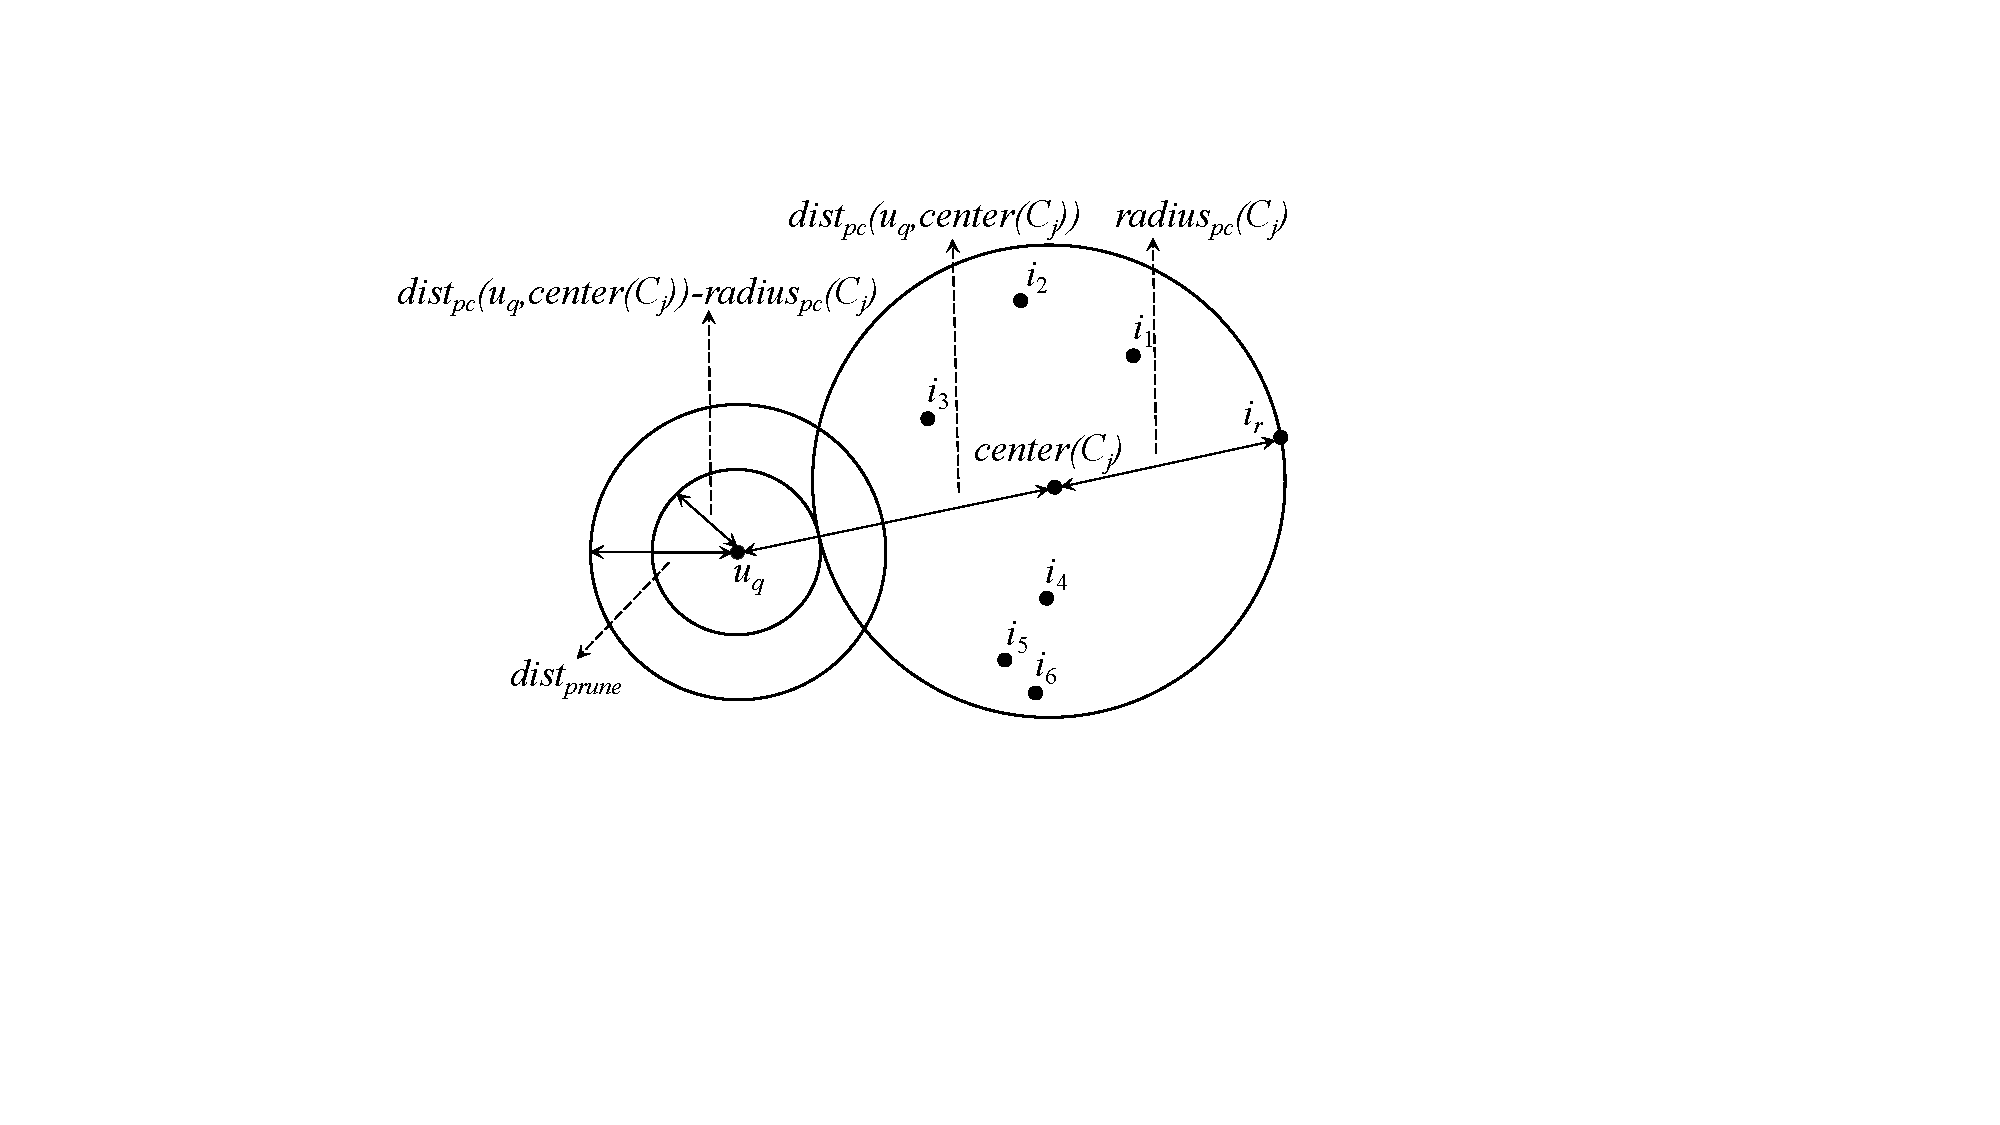
\includegraphics[width=0.41\textwidth]{Images/knn_error_11.pdf}
    \caption{Reservation of the remote data points that should be pruned in the kNN search process on \dualtree.}
    \label{fig:knn_error}
\end{figure}

Pruning in \dualtree's non-leaf nodes is performed at a coarse, cluster-level granularity. While this approach is efficient for discarding large, irrelevant portions of the search space, it is inherently \textbf{conservative}. A cluster must be retained in its entirety if its low-dimensional bounding sphere intersects the search region. That is, when $dist_{PC}(center(C_j), u)-radius_{PC}(C_j)<dist_{prune}$ (used in the \deltatree part \cite{cui2003contorting}) or $dist_{PC}(center(C_j), q) - radius_{PC}(C_j) < dist_\text{MkNN}(C_j)$ (used in the \hdrtree part \cite{yang2014continuous}), where subscript $PC$ represent the principle component space corresponding to the level of the tree accommodating the cluster $C_j$, $dist_{prune}$ represents the pruning bound for kNN search on the \deltatree, and $dist_\text{MkNN}$ represents the largest $dist_{kNN}$ value of the query points in the cluster, then, the whole cluster should be reserved. However, this condition can be misleadingly triggered even when no member points are actual candidates.

This issue arises from a \textbf{spatial misalignment}, typically occurring when a cluster's radius is inflated by a single \textbf{distant point} positioned on the far side of the cluster relative to the query, as is illustrated in Figure~\ref{fig:knn_error} where the points $i_r$, which respectively determine the large radius in the visited clusters, are positioned on the far side relative to the query points $u_q$ and $i_q$. As a result, a significant number of \textbf{false positives}---points that are actually far beyond the pruning bound---survive the initial pruning stages and are passed down to the leaf nodes. This motivates the need for an additional, fine-grained pruning step at the leaf level to efficiently filter these residual candidates before the expensive full-dimensional evaluation.

\subsection{Point-level, low-dimensional pruning }

The conservative nature of \dualtree's non-leaf level, cluster-based pruning means some distant false positives inevitably reach the leaf nodes, creating avoidable overhead for the final, full-dimensional verification. We eliminate this overhead by introducing an \textbf{intermediate, point-wise pruning stage} at the leaf level. This stage employs a low-cost, \textbf{low-dimensional distance check} to efficiently filter these residual candidates before the expensive final evaluation. The following lemma formalizes this rule.

\begin{lemma}[Symmetric Point-Wise Pruning Rule]
\label{lem:pointwise-pruning}
Let $q$ be the search origin point and $v$ be a point visited at a leaf node. The roles of $q$ and $v$, and the definition of the pruning threshold $b_p$, are symmetrically defined for both search types:
\begin{list}{\textbullet}
  {\setlength{\leftmargin}{1.5em}
   \setlength{\itemsep}{0pt}
   \setlength{\parsep}{0pt}
   \setlength{\topsep}{0pt}}
    \item \textbf{For kNN search on the \deltatree:} $q \in U$ is a query, $v \in I$ is a reference point, and $b_p$ is the current $k$-th best distance.
    \item \textbf{For RkNN search on the \hdrtree:} $q \in I$ is a reference, $v \in U$ is a query point, and $b_p$ is the stored $k$NN distance of $v$, i.e., $dist_{k\mathrm{NN}}(v)$.
\end{list}
Let $dist_{PC}$ be the distance of two points in the selected principle component space, if $dist_{P}(q,v) \ge b_p$, then $v$ can be safely pruned because $dist(q,v)\ge dist_{PC}(q,v)\ge b_p$, according to Lemma \ref{lm:pca_decrease_dist}.
\end{lemma}

In summary, this rule provides a unified mechanism to accelerate both forward kNN and reverse kNN searches by efficiently filtering false positives at the leaf nodes of both the \deltatree\ part and the \hdrtree part of the \dualtree. 

However, the effectiveness of this stage hinges on a critical question: what is the optimal projection dimensionality, $d$, to use for this check. The choice involves a fundamental trade-off: a higher $d$ offers more pruning power but incurs a greater computational cost for the check itself. To resolve this, we now develop a cost-aware mathematical model that formally relates the pruning dimensionality to the expected computational overhead, enabling us to derive the theoretically optimal value for $d$.


\begin{comment}
\stitle{Basic ANALYSIS on Pruning DimensionALITy}

It is crucial to select an appropriate number of principal component dimensions for this newly introduced low-dimensional pruning step on the leaf level of \dualtree. Because the computational overhead on the leaf level of \dualtree equipped with this new pruning step is depended on the number of pruning dimensions used. However, determining the optimal dimensionality is challenging, as it involves balancing two opposing factors that impact the amount of leaf-level computations. 

On one hand, based on the definition of Euclidean distance that $dist(A,B) = \sqrt{\sum_{i=1}^{D}(A[i] - B[i])^2}$, where $D$ is the number of dimensions, using more principal components increases the number of coordinate-wise subtraction and squaring operations in low-dimensional distance calculation for the pruning step.

On the other hand, incorporating more principal components into low-dimensional distance calculation can improve the probability of successfully pruning the points that should ideally be eliminated, as is discussed in the theorem below.

\begin{theorem}
    Let $q$ be a data point for which kNN or RkNN search is performed, and let $v$ be a visited data point at the leaf level of \dualtree during the search process of $q$. let $b_p$ denote the pruning bound and let $dist$ denote a shorthand for the (full-dimensional) distance $dist(q, v)$ between $q$ and $v$. Furthermore, define $dist_a$ and $dist_b$ as shorthand notations for $dist_a(q, v)$ and $dist_b(q, v)$, which represent the low-dimensional distances computed on the first $a$ and $b$ principal component dimensions, respectively, where $a < b$. Then,
    \begin{flalign}     
        &\text{When  } dist \geq b_p, \quad P(dist_b \geq b_p) \geq P(dist_a \geq b_p). \nonumber
    \end{flalign}
    \begin{proof}
        Let $g_a:dist\rightarrow dist_{a}$, that is, $g_a(dist)=dist_{a}$, let $g_b:dist\rightarrow dist_{b}$, that is, $g_b(dist)=dist_{b}$, and let $q_{PC}[i]$ and $v_{PC}[i]$ respectively denote the element of $q$ and $v$ on the $i$-th principle component dimension. Because $dist_{b}=\sqrt{\sum^b_{i=1}(q_{PC}[i]-v_{PC}[i])^2}$, $dist_{a}=\sqrt{\sum^a_{i=1}(q_{PC}[i]-v_{PC}[i])^2}$ and that $b>a$, it can be derived that:
        \begin{flalign}
        &g_b(dist)=dist_{b}\geq dist_{a}=g_a(dist) \nonumber \\
         \Rightarrow& \{dist|g_{a}(dist)\geq b_p\}\subset \{dist|g_{b}(dist)\geq b_p\} 
        \end{flalign}
        Hence, under the notation that $f_{dist}(x)$ represent the probability function of the distance between $q$ and $v$, the following conclusion can be drawn that:
        \begin{flalign}
            &P(dist_b\geq b_p)=\int_{\{x|g_b(x)\geq b_p\}}f_{dist}(x)dx\nonumber\\
            \geq& P(dist_a\geq b_p)=\int_{\{x|g_a(x)\geq b_p\}}f_{dist}(x)dx
        \end{flalign}
    \end{proof}
    In conclusion, using more principal component dimensions for pruning can increase the success rate of eliminating visited data points whose distances to the search-originating point exceed the pruning bound and are therefore expected to be pruned.
\end{theorem}


Based on the analysis above, the work of choosing an optimal pruning dimensionality is about achieving the best balance between pruning effect and computational overhead. In order to locate the optimal number of pruning dimensions, a theoretically grounded strategy will be proposed in the next subsection. 
\end{comment}

\noindent \textbf{COST-AWARE DIMENSIONALITY SELECTION.} 
%
The goal of selecting an optimal number of pruning dimensions is to minimize the expected computational cost for a randomly visited data point on a leaf node of \dualtree during the search process for a randomly selected search-originating data point. We first formulate a cost model that expresses the expected cost as a function of the pruning dimensionality, $d$. We then derive the optimal pruning dimensionality by applying optimization methods to this model.

While leaf-node processing involves minor operations like bound comparisons and inserting the visited point into the RkNN list or the list containing the candidate kNN members of the query origin, their computational cost in high-dimensional settings is overwhelmingly dominated by distance calculations. Our cost model therefore focuses exclusively on this dominant factor. We model the cost by defining a unit cost $c$ as the expense of a single-dimension squared difference and addition within a Euclidean distance computation. Consequently, a $d$-dimensional distance check incurs a cost of approximately $dc$.

Let $d$ be the pruning dimensionality and $D$ be the full dimensionality. For any visited point at a leaf node, there are three possible outcomes based on our pruning rule:

\noindent \underline{\textit{Situation 1}: True Candidate}: The point should be accepted. It passes the $d$-dim check and requires a full $D$-dim verification. The total cost is $(d+D)c$. This occurs with probability $P_a$.

\noindent\underline {\textit{Situation 2}: False Positive (Pruned):} The point is not a neighbor and is successfully pruned by the $d$-dim check. The cost is only $dc$. This occurs with probability $P_p(d)$.

\noindent\underline {\textit{Situation 3}: False Positive (Not Pruned):} The point is not a real kNN candidate or a RkNN member of the query origin but survives the $d$-dim check, requiring a full $D$-dim verification to be discarded. The total cost is $(d+D)c$. This occurs with probability $1 - P_a - P_p(d)$.


By summing the costs of these mutually exclusive outcomes, we derive the expected cost as a function of $d$.

\begin{lemma}[Expected Cost Model]
\label{thm:cost-model}
The expected computation cost $E_{cost(q,v)}(d)$ for processing a visited leaf-node is given by $E_{cost(q,v)}(d)=(D-D\cdot P_p(d)+d)c$, which is a direct simplification of the full expectation $E = P_a(d+D)c + P_p(d)dc + (1-P_a-P_p(d))(d+D)c$.
\end{lemma}

To minimize this cost, our central challenge reduces to accurately modeling the pruning probability function, $P_p(d)$. To develop a tractable model for this function, we assume that the data distribution remains relatively stable throughout the update process and formalize the statistical properties of the process below.

\paragraph{Notation}
Before detailing these properties, we define the minimal bounding hyperrectangles, $\mathcal{O}_U$ and $\mathcal{O}_I$, that respectively enclose all points of $U$ and $I$ during the update process:
\begin{align}
    \mathcal{O}_U &= \{P \mid \forall j\in[1,D], u[j]_{\min} \le P[j] \le u[j]_{\max}\} \\
    \mathcal{O}_I &= \{P \mid \forall j\in[1,D], i[j]_{\min} \le P[j] \le i[j]_{\max}\}
\end{align}
Here, $u[j]_{\min}$, $u[j]_{\max}$ and $i[j]_{\min}$, $i[j]_{\max}$ are respectively the minimum and maximum coordinates observed in the set $U$ and $I$ during the update process. For subsequent discussions, we use $\mathcal{O}$ as a collective term for both $\mathcal{O}_U$ and $\mathcal{O}_I$ when the context is clear.

We assume that, during the update period, There exist the following objects:

\noindent (1). a partition of $\mathcal{O}$ into $M$ sub-spaces that $\mathcal{O} = \bigcup_{i=1}^{M}\mathcal{O}^i$.

\noindent (2). a sequence of probability values $P_i$ for $1 \leq i \leq M$.

\noindent (3). a sequence of positive integers $B_i$ for $1 \leq i \leq M$.

\noindent (4). $M$ lists of probability values, where the $i$-th list contains $B_i$ probability values denoted by $\pi_{ij}$ for $1 \leq i \leq M,\, 1 \leq j \leq B_i$, with $\pi_{ij}$ representing the $j$-th probability value in the $i$-th list.

\noindent (5). $M$ lists of probability density functions, where the $i$-th list contains $B_i$ density functions denoted by $f_{ij}$ for $1 \leq i \leq M,\, 1 \leq j \leq B_i$, with $f_{ij}$ representing the $j$-th distribution in the $i$-th list.

 These objects ensures that the following properties hold throughout the update process. Note that the notation $\mathcal{O}$ is used in this paper as a collective reference to both $\mathcal{O}_U$ and $\mathcal{O}_I$, which does not imply that $\mathcal{O}_U = \mathcal{O}_I$. When $\mathcal{O} = \mathcal{O}_U$ and $\mathcal{O}_I$, respectively, the aforementioned objects may differ.


\noindent \underline{PROPERTY 1}: For a randomly selected search-originating point $q$, the probability of $q$ to be included in $O^i$ is approximately equal to $P_i$, that is $P(q\in \mathcal{O}^i)\approx P_i$. 

\noindent \underline{PROPERTY 2}: When $\mathcal{O}=\mathcal{O}_{U}$, for a random point $q$, if $q\in \mathcal{O}^i$, the number of distinct pruning bound values the search process of $q$ passes through is $B_i$. And when $\mathcal{O}=\mathcal{O}_{I}$, if the data point $q$ requiring RkNN Search belongs to $\mathcal{O}^i$, the pruning bound values the search process of $q$ passes through tend to cluster around $B_i$ distinct values. In this paper, we refer to these representative values, around which the pruning bound values concentrate, as \emph{bound kernels}.

\noindent \underline{PROPERTY 3}: For a random visited data point $v$ on the leaf level of \dualtree  during the search process of a random data point $q$, the conditional probability that $v$ encounters the $j$-th ( $1\leq j\leq B_i$) pruning bound value (bound kernel) $b_{p}(q,j)$ for the search of $q$ that $b_p=b_{p}(q, j)$ when $q\in \mathcal{O}^i$ is given by $P(b_p=b_{p}(q, j)|q\in \mathcal{O}^i)\approx \pi_{ij}$. 

\noindent \underline{PROPERTY 4}: Let $q_{\mathcal{O}^i}$ be an arbitrary search origin in $\mathcal{O}^i$ and $v^{j}_{q_{\mathcal{O}^i}}$ be a random visited data point encountering the $j$-th pruning bound (bound kernel) $b_{p}(q_{O^i},j)$ for the search of $q_{O^i}$, and treat $q_{O^i}$ as a fixed point when computation for the square rate $dist^{2}(q_{\mathcal{O}^i},v^{j}_{q_{\mathcal{O}^{i}}})/b^{2}_{p}(q_{O^i},j)$. Note that $dist^{2}(q_{\mathcal{O}^i},v^{j}_{q_{\mathcal{O}^{i}}})/b^{2}_{p}(q_{O^i},j)$ is a random variable because $v$ is randomly selected. Then, the probability density function $f_{dist^{2}(q_{\mathcal{O}^i},v^{j}_{q_{\mathcal{O}^{i}}})/b^{2}_{p}(q_{O^i},j)}(q_{\mathcal{O}^i},x)$  shows minimal sensitivity to the specific position of $q_{\mathcal{O}^i}$ within $\mathcal{O}^i$, and is approximately equal to $f_{ij}$, which is a constant distribution. Hence, the density function $f_{dist^{2}(q_{\mathcal{O}^i},v^{j}_{q_{\mathcal{O}^{i}}})/b^{2}_{p}(q_{O^i},j)}(q_{\mathcal{O}^i},x)$ can also be written as $f_{dist^{2}(q_{\mathcal{O}^i},v^{j}_{q_{\mathcal{O}^{i}}})/b^{2}_{p}(q_{O^i},j)}(x)$. In conclusion, the following approximation can be deduced that: 

\begin{flalign}
&f_{(dist^2(q,v)/b_p^2 |q\in \mathcal{O}^i ;b_p=b_{p}(q,j))}\approx f_{dist^2(q_{\mathcal{O}^i},v^{j}_{q_{\mathcal{O}^i}})/b^{2}_{p}(q_{O^i},j)}\approx f_{ij}  
\label{equ: local_distribution}
\end{flalign}

In the approximation above,  $f_{(dist^2(q,v)/b_p^2 |q\in \mathcal{O}^i ;b_p=b_{p}(q,j))}$ represents the probability density function of the random variable $dist^2(q,v)/b_p^2$ where both $q$ and $v$ are random data points under the condition that $q\in \mathcal{O}^i$ and $v$ encounters the $j$-th pruning bound(bound kernel) that $b_p=b_{p}(q,j)$. For convenient expression, the term \textbf{local distribution} is used to uniformly refer to $f_{(dist^2(q,v)/b_p^2 |q\in \mathcal{O}^i ;b_p=b_{p}(q,j))}$, $f_{dist^2(q_{\mathcal{O}^i},v^{j}_{q_{\mathcal{O}^i}})/b^{2}_{p}(q_{O^i},j)}$, and $f_{ij}$ in the following discussion, which are three equivalent distributions because of property 4.  


Based on the settings and conditions given before, the function $P_p(d)$ can now be analyzed. As discussed earlier, $P_p(d)$ represents the probability that $v$ should not be included in either the RkNN list or the candidate kNN list of $q$, and can be pruned through low-dimensional distance computation. This leads to the following deduction.
\begin{flalign}
P_p(d)&=P(dist_{PC}(q,v)\geq b_p)=P(\frac{dist^2(q,v)}{b_p^2}\geq \frac{dist^2(q,v)}{dist_{PC}^2(q,v)})  
\label{equ: ped_basic}
\end{flalign}
Given the deduction above, the density function $f_{dist^2(q,v)/b_p^2}$ of the random variable $dist^2(q,v)/b_p^2$ and the relationship between $d$ and $dist^2(q,v)/dist_{PC}^2(q,v)$ should be further studied in order to formulate $P_p(d)$. For convenient expression, we use the term \textbf{global distribution} to refer to the distribution of the random variable $dist^2(q,v)/b_p^2$ in the subsequent content.







\begin{comment}
\stitle{Cost for a visited point}

As previously discussed in the new pruning step and reflected in Algorithms~\ref{alg:RKNNSearch} and~\ref{alg:knnsearch} for RkNN and kNN search on \dualtree, given a random visited point in a leafnode in the search process for a random query point, the computation might include three parts, which are distance computation, judgment of the relationship between the distance and the bound value and the operation of inserting the visited point into the RkNN list or the list containing the candidate kNN members of the query point. Compared to the operation of judgment and insertion, distance computation is more time-consuming because of being in high-dimensional Euclidean space, therefore accounting for the majority of the total computation time cost. As a result, when estimation of the computation time cost of a visited point in this paper, only the time cost for distance computation is considered. 

\begin{definition}
In this work, we explicitly define $c$ as the total cost of computing the squared difference for each dimension followed by one addition operation with the squared difference of its immediate subsequent dimension in the calculation of Euclidean distance that $dist(A,B)=\sqrt{\sum^{D}_{i=1}(A[i]-B[i])^2}$ is defined as $c$.

\label{def: cost_unit}
\end{definition}

According to Definition \ref{def: cost_unit}, the computational cost of calculating a $d$-dimensional Euclidean distance in this context can be approximately estimated as $dc$. It should be noted that our approximate estimation of computational cost includes one additional addition operation compared to the actual computational overhead, as no further addition follows the squared difference calculation for the final dimension when computing the Euclidean distance. At the same time, our computational cost estimation omits one square-root operation compared to the actual cost. Nevertheless, due to the high-dimensional context of this work, the extra addition and the excluded square-root operation can be considered negligible relative to the many addition and squared difference calculations encompassed by $dc$.

\leveltwo{General Model of the Cost}

Given that the full dimensionality of the Euclidean space where \fdknnj is implemented is $D$, and that the applied pruning dimensionality in the new step added to the search algorithm for the leafnodes is $d$, then, for a random visited point at leafnodes within the search process on \dualtree of a random query point, there exist three situations.

\noindent \underline{\textit{Situation 1}}: The visited point is a point that should be accepted, whose exact distance to the query point is smaller than the pruning bound value. In this case, the visited point can get through the initial $d$-dimensional pruning and full($D$)-dimensional distance is needed to identify it. As a result, the computation cost needed should be $(D+d)c$. For a random visited point at the leafnodes, the probability for it to be within the bound from the query point is noted as $P_a$ in this paper.

\noindent\underline {\textit{Situation 2}}: The visited point is a point that should not be accepted and can be excluded by the initial $d-$dimensional pruning. In this case, the computation cost needed should be $dc$. For a random visited point at the leafnodes, the probability for it to be pruned by $d-$dimensional distance computation is depended on the value of $d$. A larger $d$ provides a low-dimensional distance closer to the full-dimensional distance, thus, the probability for the low-dimensional distance to exceed the pruning bound value would be higher and it is more likely for the visited point to be identified by the $d$-dimensional pruning. As a result, the probability for a visited point to be pruned is a function of $d$, denoted as $P_{p}(d)$ in this paper.

\noindent \underline{\textit{Situation 3}}: The visited point is a point that should not be accepted but still can get through the initial $d-$dimensional pruning and full($D$)-dimensional distance is needed to identify it. In this case, the computation cost needed should be $(D+d)c$. For a random visited point at the leafnodes, the probability that it should be excluded but can get through the initial low($d$)-dimensional pruning should be $1-P_a-P_p(d)$ in this paper.

Based on the analysis above, a theorem can be established as below:
\begin{theorem}{(General Model of the cost for a visited data point).} In a Eucliean Space whose full number of dimensions is $D$, given an applied pruning dimensionality $d$ and a randomly selected visited data point $v$ on the leaf level of \dualtree in the search process for a randomly selected search-originating point $q$, the expectation value $E_{cost(q,v)}(d)$ of the computation cost $cost(q,v)$ for processing $v$ can be derived by the formula below.
\begin{flalign}
    E_{cost(q,v)}(d)=(D-D\cdot P_p(d)+d)c \IEEEyesnumber
    \label{equ: cost_visited_point}
\end{flalign}
\label{thm:cost_one_visited_point}
\end{theorem}

\begin{proof}
According the three possible situations discussed earlier, 
\begin{flalign}
    E_{cost(q,v)}(d) &= P_a(D+d)c+d\cdot P_p(d)c    \IEEEnonumber \\
    &+(1-P_a-P_p(d))(D+d)c              \IEEEyesnumber
    \label{equ: proof_cost_visited_point}
\end{flalign}
Therefore, $E_{cost(q,v)}(d)=(D-D\cdot P_p(d)+d)c$

\end{proof}
\noindent Theorem \ref{thm:cost_one_visited_point} gives a general model to compute the expected computation cost $E_{cost(q,v)}(d)$ for a randomly selected data point $v$ visited on leaf level within the search process for a randomly selected search-originating data point $q$. In the formula given, the full dimensionality $D$ is treated as a fixed constant number, as a result, what remains for determination of the optimal pruning dimensionality to minimize $E_{cost(v,q)}(d)$ is to formulate the function $P_p(d)$ for the pruning probability.
\end{comment}






\begin{comment}

\leveltwo{Function of Pruning Dimensionality and rate}
\begin{comment}
Before analysis of the function $P_p(d)$ between the pruning probability and the pruning dimensionality, it is important to clarify that the approach proposed later in this paper is designed to derive $P_p(d)$ under a stable phase, during which the fluctuation in $P_p(d)$ is negligible. Similar to the strategy for maintaining the performance of the \dualtree index by efficiency monitoring and reconstruction introduced in the previous section, the efficiency of the \dualtree index, equipped with the new pruning step, should also be monitored using the same method. If its performance falls below a specified threshold, both the tree index and the function $P_p(d)$ need to be re-computed. 

Given that general data distribution evolves only slightly in a stable phase, and to simplify the deduction process, one additional condition is assumed for the stable phase, alongside the condition 1 to condition 3 proposed in the part of RECONSTRUCTION OF Dual-Tree in last section. When in practical scenario, we still use condition 3 to identify whether a stable phase has ended. The results presented in the experiment section will demonstrate that the \dualtree index, enhanced by the pruning step applied at the leaf nodes with the optimal dimensionality computed based on the conditions of stable phase set in this paper, can maintain consistently high efficiency even after a significant number of updates. 

Before introduction of the new condition, in order to simplify the subsequent discussion, We use the symbol $\mathcal{O}$ as a collective term for both $\mathcal{O}_U$ and in this paper, $\mathcal{O}_I$. $\mathcal{O}_U$ and $\mathcal{O}_I$ are used to represent the smallest $D$-dimensional Euclidean spaces respectively covering $U$ and $I$ during the whole stable phase that
\begin{flalign}
&\mathcal{O}_U=\{P|u[j]_{min}\leq P[j]\leq u[j]_{max}, u \in U, 1\leq j\leq D\}\\ \yesnumber
&\mathcal{O}_I=\{P|i[j]_{min}\leq P[j]\leq i[j]_{max}, i\in I, 1\leq j\leq D\}         \yesnumber
\end{flalign}
where $P$ means a data point, $u$ and $i$ respectively means an arbitrary data point in $U$ and $I$ during the stable phase, $u[j]_{max}$, $u[j]_{min}$, $i[j]_{max}$, and $i[j]_{min}$ respectively represent the maximal and minimal values of the data points in $U$ and $I$ along the $j$-th dimension throughout the entire stable phase.





\noindent \underline{\textit{Condition 3}}:  

There exist the following objects:
\begin{enumerate}
    \item a partition of $\mathcal{O}$ into $M$ sub-spaces that $\mathcal{O} = \bigcup_{i=1}^{M}\mathcal{O}^i$.
    \item  a sequence of probability values $P_i$ for $1 \leq i \leq M$.
    \item  a sequence of positive integers $B_i$ for $1 \leq i \leq M$.
    \item  $M$ lists of probability values, where the $i$-th list contains $B_i$ probability values denoted by $\pi_{ij}$ for $1 \leq i \leq M,\, 1 \leq j \leq B_i$, with $\pi_{ij}$ representing the $j$-th probability value in the $i$-th list.
    \item  $M$ lists of probability density functions, where the $i$-th list contains $B_i$ density functions denoted by $f_{ij}$ for $1 \leq i \leq M,\, 1 \leq j \leq B_i$, with $f_{ij}$ representing the $j$-th distribution in the $i$-th list.
\end{enumerate}
 These objects ensures that the following properties hold throughout the entire stable phase. Note that the notation $\mathcal{O}$ is used in this paper as a collective reference to both $\mathcal{O}_U$ and $\mathcal{O}_I$, which does not imply that $\mathcal{O}_U = \mathcal{O}_I$. When $\mathcal{O} = \mathcal{O}_U$ and $\mathcal{O}_I$, respectively, the aforementioned objects may differ.


\noindent PROPERTY 1: During the whole stable phase, for a randomly selected search-originating point $q$, the probability of $q$ to be included in $O^i$ is approximately equal to $P_i$, that is $P(q\in \mathcal{O}_i)\approx P_i$. 

\noindent PROPERTY 2: When $\mathcal{O}=\mathcal{O}_{U}$, for a random point $q$, if $q\in \mathcal{O}^i$, the number of distinct pruning bound values the search process of $q$ passes through is $B_i$. And when $\mathcal{O}=\mathcal{O}_{I}$, if the data point $q$ requiring RkNN Search belongs to $\mathcal{O}^i$, the pruning bound values the search process of $q$ passes through tend to cluster around $B_i$ distinct values. In this paper, we refer to these representative values, around which the pruning bound values concentrate, as \emph{bound kernels}.

\noindent PROPERTY 3: For a random visited data point $v$ on the leaf level of \dualtree  during the search process of a random data point $q$, the conditional probability that $v$ encounters the $j$-th ( $1\leq j\leq B_i$) pruning bound value (bound kernel) $b_{p}(q,j)$ for the search of $q$ that $b_p=b_{p}(q, j)$ when $q\in \mathcal{O}^i$ is given by $P(b_p=b_{p}(q, j)|q\in \mathcal{O}^i)\approx \pi_{ij}$. 

\noindent PROPERTY 4: Let $q_{\mathcal{O}^i}$ be an arbitrary search-originating point in $\mathcal{O}^i$ and $v^{j}_{q_{\mathcal{O}^i}}$ be a random visited data point encountering the $j$-th pruning bound (bound kernel) $b_{p}(q_{O^i},j)$ for the search of $q_{O^i}$, and treat $q_{O^i}$ as a fixed point when computation for the square rate $dist^{2}(q_{\mathcal{O}^i},v^{j}_{q_{\mathcal{O}^{i}}})/b^{2}_{p}(q_{O^i},j)$ between the distance $dist(q_{\mathcal{O}^i},v^{j}_{q_{\mathcal{O}^{i}}})$ between $q_{O^i}$ and $v^{j}_{q_{\mathcal{O}^i}}$ and $b_{p}(q_{O^i},j)$. Note that $dist^{2}(q_{\mathcal{O}^i},v^{j}_{q_{\mathcal{O}^{i}}})/b^{2}_{p}(q_{O^i},j)$ is a random variable because $v$ is randomly selected. Then, the probability density function $f_{dist^{2}(q_{\mathcal{O}^i},v^{j}_{q_{\mathcal{O}^{i}}})/b^{2}_{p}(q_{O^i},j)}(q_{\mathcal{O}^i},x)$ of $dist^{2}(q_{\mathcal{O}^i},v^{j}_{q_{\mathcal{O}^{i}}})/b^{2}_{p}(q_{O^i},j)$ shows minimal sensitivity to the specific position of $q_{\mathcal{O}^i}$ within $\mathcal{O}^i$, and is approximately equal to $f_{ij}$.  In another term, regardless of the specific position of $q_{\mathcal{O}^i}$, $f_{dist^{2}(q_{\mathcal{O}^i},v^{j}_{q_{\mathcal{O}^{i}}})/b^{2}_{p}(q_{O^i},j)}(q_{\mathcal{O}^i},x)$ is approximately equal to $f_{ij}$, which is a constant distribution. Hence, $f_{dist^{2}(q_{\mathcal{O}^i},v^{j}_{q_{\mathcal{O}^{i}}})/b^{2}_{p}(q_{O^i},j)}(q_{\mathcal{O}^i},x)$ can also be written as $f_{dist^{2}(q_{\mathcal{O}^i},v^{j}_{q_{\mathcal{O}^{i}}})/b^{2}_{p}(q_{O^i},j)}(x)$. In conclusion, the following approximation can be deduced that: 

\begin{flalign}
&f_{(dist^2(q,v)/b_p^2 |q\in \mathcal{O}^i ;b_p=b_{p}(q,j))}\approx f_{dist^2(q_{\mathcal{O}^i},v^{j}_{q_{\mathcal{O}^i}})/b^{2}_{p}(q_{O^i},j)} \nonumber\\
&\approx f_{ij}  \IEEEyesnumber
\label{equ: local_distribution}
\end{flalign}

In the approximation above,  $f_{(dist^2(q,v)/b_p^2 |q\in \mathcal{O}^i ;b_p=b_{p}(q,j))}$ means the probability density function of the random variable $dist^2(q,v)/b_p^2$ where both $q$ and $v$ are random data points under the condition that $q\in \mathcal{O}^i$ and $v$ encounters the $j$-th pruning bound(bound kernel) that $b_p=b_{p}(q,j)$. For convenient expression, in the following discussion, the term \textbf{local distribution} is used to uniformly refer to $f_{(dist^2(q,v)/b_p^2 |q\in \mathcal{O}^i ;b_p=b_{p}(q,j))}$, $f_{dist^2(q_{\mathcal{O}^i},v^{j}_{q_{\mathcal{O}^i}})/b^{2}_{p}(q_{O^i},j)}$, and $f_{ij}$, which are three equivalent distributions under property 4.  
\end{comment}

\begin{comment}
Based on the settings and conditions given before, the function $P_p(d)$ can now be analyzed. As discussed earlier, $P_p(d)$ represents the probability that $v$ should not be included in either the RkNN list or the candidate kNN list of $q$, and can be pruned through low-dimensional distance computation. This leads to the following deduction.
\begin{flalign}
P_p(d)&=P(dist_{PC}(q,v)\geq b_p)  \nonumber \\
&=P(\frac{dist^2(q,v)}{b_p^2}\geq \frac{dist^2(q,v)}{dist_{PC}^2(q,v)})  
\label{equ: ped_basic}
\end{flalign}
Given the deduction above, the probability density function $f_{dist^2(q,v)/b_p^2}$ of the random variable $dist^2(q,v)/b_p^2$ and the relationship between $d$ and $dist^2(q,v)/dist_{PC}^2(q,v)$ should be further studied in order to formulate $P_p(d)$. For convenient expression, we use the term \textbf{global distribution} to refer to the distribution of the random variable $dist^2(q,v)/b_p^2$ in the subsequent content.
\end{comment}

\noindent\textbf{Distance Shrinkage and Pruning Dimensionality}: To investigate the functional relation between the pruning dimensionality and the square rate $dist^2(q,v)/dist^2_{PC}(q,v)$ between the full-dimensional distance and the low-dimensional distance computed on a part of principle component dimensions, which is the distance shrinkage effect of dimensional reduction by PCA, we revisit the properties of PCA and observe that, the eigenvalue $e_i$ of the co-variance matrix of the initial state of $U\cup I$ before the update starts corresponding to the $i$th row vector of the PCA projection matrix $M$ is equal to the variance $\sigma^2_i$ of the elements of the data points in initial $U\cup I$ along the $i$th dimension $PC(i)$ of the PC space. And $\sigma^2_i$, defined as $\frac{\sum_{p\in U\cup I}(p_{PC(i)}-\overline{p_{PC(i)}})^2}{|U\cup I|}$, represents the degree of dispersion of the data points along such dimension. Consequently, given the pruning dimensionality $d$ and the number of full dimensions $D$, the following approximation can be made reasonably that:
\begin{flalign}
    \frac{dist^2(v,q)}{dist_{PC}^2(v,q)}\approx\frac{\sum_{i=1}^{D}\sigma^2_i}{\sum_{i=1}^{d}\sigma^2_i}= \frac{\sum_{i=1}^{D}e_i}{\sum_{i=1}^{d}e_i} 
\end{flalign}

Because the row vectors in the PC matrix are sorted in descending order according to their corresponding eigenvalues, the speed of increasing of $ \frac{\sum_{i=1}^{d}e_i}{\sum_{i=1}^{D}e_i}$ is fast when $d$ is small and turn slower as $d$ increases, forming a curve that rises sharply first and tends to be flat in the coordinate system whose X-axis represents $d$ and Y-axis represents $ \frac{\sum_{i=1}^{d}e_i}{\sum_{i=1}^{D}e_i}$. Therefore, a function that $\frac{\sum_{i=1}^{d}e_i}{\sum_{i=1}^{D}e_i}\approx kln(d)+b$, which forms a similar function graph, can be used to approximately estimate the relationship between $ \frac{\sum_{i=1}^{d}e_i}{\sum_{i=1}^{D}e_i}$ and $d$. As a result, the functional model $kln(d)+b$ can also be applied for $dist_{PC}^2(q,v)/dist^2(q,v)$, which can be written in the following mathematical form that
\begin{flalign}
    \frac{dist_{PC}^2(v,q)}{dist^2(v,q)}\approx \frac{\sum_{i=1}^{d}e_i}{\sum_{i=1}^{D}e_i}\approx kln(d)+b 
\end{flalign}

Given the approxiamte function of $dist^2(q,v)/dist^2_{PC}(q,v)$, what remains to achieve are the two parameters $k$ and $b$. Parameters $k$ and $b$ can be located by the following two pairs of values of $d$ and $\frac{\sum_{i=1}^{d}e_i}{\sum_{i=1}^{D}e_i}$, that is:
\begin{flalign}
&kln(d)+b=b=\frac{e_1}{\sum_{i=1}^{D}e_i} \quad \text{when } d=1 \\
&kln(d)+b=kln(D)+b=\frac{\sum_{i=1}^{D}e_i}{\sum_{i=1}^{D}e_i}=1 \quad \text{when } d=D
\end{flalign}

In this stage with the parameters $k$ and $b$ are obtained, the function between the pruning dimensionality and the square rate between the full-dimensional and low-dimensional distance is derived.
\begin{comment}
In conclusion, the linear-log model that $kln(d)+b$ is observed to match the functional model of the relationship between the pruning dimensionality and the square rate $dist^2(q,v)/dist^2_{PC}(q,v)$ between the full-dimensional distance and the low-dimensional distance. And the proportions $\sum^d_{i=1}e_i/\sum^D_{i=1}e_i$ of the first $d$ eigen values in the sum of all the eigen values of the co-variance matrix of the initial $U\cup I$ across different $d$ values are collected before the update happens. Then, these proportions are applied to derive the two parameters $k$ and $b$ in the model $kln(d)+b$. The estimation of the parameters is at the beginning of a stable phase before the update starts, according to condition 1 of a stable phase, the parameters estimated can keep effective for a long phase, which can be verified by the experiment results in this paper. And once the efficiency of \dualtree equipped with the new pruning step is observed to be lower than the threshold specified in condition 3, the function between $dist^2(q,v)/dist^2_{PC}(q,v)$ should be re-computed.
\end{comment}
In order to achieve the function between pruning dimensionality and the pruning probability, the global distribution will be discussed in what follows. 

\begin{comment}
\noindent\textbf{Distance Shrinkage and Pruning Dimensionality}: Based on the properties of PCA, the cumulative energy of the eigenvalues---the term $\sum_{i=1}^{d}e_i / \sum_{i=1}^{D}e_i$---exhibits a logarithmic growth pattern as $d$ increases. We therefore propose to approximate the distance shrinkage ratio with a simple yet effective log-linear model:
\begin{align}
    \frac{\mathrm{dist}^2(v,q)}{\mathrm{dist}_{PC}^2(v,q)} \approx \frac{\sum_{i=1}^{D}e_i}{\sum_{i=1}^{d}e_i} \approx k\ln(d)+b
    \label{eq:shrinkage-model}
\end{align}

The model's parameters, $k$ and $b$, are uniquely determined by solving the system of two linear equations defined by the boundary conditions at $d=1$ and $d=D$:
\begin{flalign}
    &k\ln(1)+b = \frac{\sum_{i=1}^{D}e_i}{e_1} \implies b = \frac{\sum_{i=1}^{D}e_i}{e_1} \nonumber \\
    &k\ln(D)+b = 1
\end{flalign}
With parameters $k$ and $b$ thus determined, we obtain a complete, closed-form model for the distance shrinkage ratio as a function of the pruning dimensionality $d$. This model is a critical component for estimating the pruning probability, $P_p(d)$, which we discuss next.
\end{comment}


\noindent\textbf{Global Distribution:} We use the technique of statistic inference, which is the commonly used approach to approximate the global distribution. Formulation of $f_{dist^2(q,v)/b^2_p}$ can be accomplished by two steps, which are deriving the probability model of $dist^2(q,v)/b^2_p$ and confirming the parameters in the probability model.


\noindent\textbf{Model of global distribution}: According to the law of total probability and Bayes' Theorem and the conditions assumed before, the theorem  below can be obtained.
\begin{lemma}{(Model of global distribution).}
Global distribution is a linear combination of local distributions, in mathematical form, it can be written as:
$f_{dist^2(q,v)/b^2_p}\approx \sum^{M}_{i=1}\sum^{B_i}_{j=1} P_i\pi_{ij}f_{ij}$   
\end{lemma}
\label{thm:framework_F}
\begin{proof}
Because of the Law of Total Probability, the approximation below holds throughout the update process:
\begin{flalign}
f_{dist^2(q,v)/b^2_p}&=\sum^{M}_{i=1}P(q\in \mathcal{O}^i)f_{(dist^2(q,v)/b^2_p|q\in \mathcal{O}^i)} \nonumber   \\
&\approx \sum^{M}_{i=1}P_if_{(dist^2(q,v)/b^2_p|q\in \mathcal{O}^i)}  
\label{equ:F_general_domain_partiton}
\end{flalign}

Because of the Law of Total Probability and the property 2,3,4 assumed, the below approximation holds throughout the update process.
\begin{flalign}
&f_{(dist^2(q,v)/b^2_p|q\in \mathcal{O}^i)} \nonumber \\
&=\sum^{B_i}_{j=1} P(b_p=b_p(q,j)|q\in \mathcal{O}^i)f_{(dist^2(q,v)/b^2_p|b_p=b_p(q,j);q\in \mathcal{O}^i)}  \nonumber  \\
&\approx \sum^{B_i}_{j=1} \pi_{ij}f_{ij} 
\label{equ:F_general_pruningboundpartition}
\end{flalign}
Therefore, $f_{dist^2(q,v)/b^2_p}\approx \sum^{M}_{i=1}\sum^{B_i}_{j=1} P_i\pi_{ij}f_{ij}$ holds during the update process.
\end{proof}




As a result, in order to achieve the global distribution that is the probability distribution of $dist^2(q,v)/b^2_p$, it is necessary to formulate $f_{ij}$ with $1\leq i\leq M$ and $1\leq j \leq B_i$.

According to property 4, $f_{dist^2(q_{\mathcal{O}^i},v^{j}_{q_{\mathcal{O}^i}})/b^{2}_{p}(q_{O^i},j)} \approx f_{ij}$ regardless of the specific position of $q_{\mathcal{O}^i}$ in $\mathcal{O}^i$. 

Therefore, $f_{dist^2(q_{\mathcal{O}^i},v^j_{q_{O^i}})/b^{2}_p(q_{O^i},j)}$, which is a local distribution where $q_{\mathcal{O}^i}$ is an arbitrary data point in $\mathcal{O}^i$ but treated as a fixed point in the process of producing $dist^2(q_{\mathcal{O}^i},v^{j}_{q_{\mathcal{O}^i}})$ while $v^{j}_{q_{\mathcal{O}^i}}$ is a random visited point encountering the $j$-th pruning bound (bound kernel) value of the search of $q_{\mathcal{O}^i}$, can be analyzed to formulate the model of the global distribution that is the distribution of $dist^2(q,v)/b^2_p$.

We propose the following Lemma:


\begin{lemma}{(Local distribution.)}
Local distribution is approximately a Normal Distribution, which can be written in mathematical form as: $\frac{dist^2(q_{\mathcal{O}^i},v^{j}_{q_{\mathcal{O}^i}})}{b^2_{p}(q_{O^i},j)} \sim \mathcal{N}(\mu, \sigma^2), \, \text{approximately}$. 

\label{thm:normal_distribution_local}
\end{lemma}
The proof for lemma \ref{thm:normal_distribution_local} is presented in Appendix A.1 and A.2.

 As a result, global distribution, which is the distribution of $dist^2(q,v)/b_{p}^2$, is a Mixed Normal Distribution. And the density function of $dist^2(q,v)/b_{p}^2$ can be formulated as follows:
\begin{flalign}
f_{dist^2(v,q)/b_{p}^2}(x)\approx \sum^{T}_{m=1}p_m\times \frac{1}{\sqrt{2\pi\sigma^2_m}}\exp \left(-\frac{(x-\mu_m)^2}{2\sigma^2_m}\right) 
\end{flalign}
 \begin{comment}
\begin{flalign}
f_{dist^2(v,q)/b_{p}^2}(x)\approx& \sum^{T}_{m=1}p_mf_m\nonumber \\=& \sum^{T}_{m=1}p_m\times \frac{1}{\sqrt{2\pi\sigma^2_m}}\exp \left(-\frac{(x-\mu_m)^2}{2\sigma^2_m}\right) 
\end{flalign}
\end{comment}
where $T=\sum^{M}_{i=1}B_i$, and $\mu_m$ and $\sigma^2_{m}$ are respectively the expected value and variance of the $m$-th Normal Distribution.

After formulation of the distribution model of $dist^2(q,v)/b_{p}^2$, the parameters in the model should be further estimated to derive the concrete $f_{dist^2(q,v)/b_{p}^2}(x)$. The detailed discussion is presented in Appendix A.3


At this stage of the paper, we have derived the relationship between the pruning dimensionality $d$ and $dist^2(v,q)/dist^2_{PC}(v,q)$, the square rate between the full-dimensional distance $dist^2(q,v)$ and the low-dimensional distance $dist^2_{PC}(q,v)$ computed on a front part of principle component dimensions of the search-originating point $q$ and the visited point $v$. And the approximate global distribution which is the approximate distribution of $dist^2(q,v)/b^2_p$ also has been derived. Following this, the function for the pruning probability $P_{p}(d)$, which is equal to the probability that $dist^2(v,q)/b^2_p\geq dist^2(v,q)/dist_{PC}^2(v,q)$ can be obtained in the following deduction:







\begin{flalign}
&P_p(d)= \int_{\frac{dist^2(v,q)}{dist^2_{PC}(v,q)}}^{+\infty} f_{\frac{dist^2(v,q)}{b^2_p}}(x)dx\nonumber\\
\approx&\int_{\frac{1}{kln(d)+b}}^{+\infty} \sum^{T}_{m=1}p_m\times \frac{1}{\sqrt{2\pi\sigma^2_m}}\exp \left(-\frac{(x-\mu_m)^2}{2\sigma^2_m}\right)dx \label{equ:ppd}
\end{flalign}
Afterward, the optimal $d$ can be determined by finding the extremum of $E_{cost(q,v)}(d)$ to achieve minimization.

\noindent \textbf{Simplified pruning probability.} Before derivation of the extremum of $E_{cost(q,v)}(v)$, we introduce a simplified method to compute an approximate of the function $P_p(d)$ between the pruning probability and the pruning dimensionality. While this simplified approach provides a less precise relationship than the more rigorous method discussed earlier, experimental results show that the optimal pruning dimensionality derived from it still delivers satisfactory computational efficiency.

The proportion the variance along the first $d$ principle component dimensions accounts for in the sum of variance of all the dimensions is of positive relationship with the pruning probability, because higher variance proportion represents more distance information reserved. Heuristically, it can be reasonably assumed that the pruning probability $P_p(d)$ is of positive linear relationship with $\sum^{d}_{i=1}e_i/\sum^{D}_{i=1}e_i$, which can be approximately estimated by the functional model of $kln(d)+b$. As a result, the model below can be applied to approximate $P_p(d)$:
\begin{flalign}
    P_p(d)&\approx k'(kln(d)+b)+b'=k'kln(d)+k'b+b'\nonumber\\
    &\approx k''ln(d)+b'' \quad \text{where }k''=k'k,\text{ and }b''=k'b+b'\label{equ:simppd} 
\end{flalign}

The parameters $k''$ and $b''$ can be estimated by a sampling method. For the pruning probability at leafnodes of the \deltatree part of \dualtree, before the update starts, $10\%$ data points at each leafnode of the \hdrtree part should be sampled, and kNN Search for them using two different pruning dimensions $d_1$ and $d_2$ should be implemented on initial $I$, and the two pruning frequencies $P^1_p$ and $P^2_p$ should be recorded. Subsequently, the equation system below can be use to determine $k''$ and $b''$:
\begin{flalign}
    P^1_p=k''ln(d_1)+b'' \quad
    P^2_p=k''ln(d_2)+b''
\end{flalign}
    
And for the pruning probability at leafnodes of the \hdrtree part of \dualtree, at the beginning of the update starts, $10\%$ data points at each leafnode of the \deltatree part should be sampled and RkNN Search for them using two different pruning dimensions $d_1$ and $d_2$ should be implemented on initial $U$ and the two pruning frequencies $p^1_e$ and $p^2_e$ should be recorded. Subsequently, the same equation system presented above can be used to confirm $k''$ and $b''$.

In conclusion, a simplified linear-log model that $k''ln(d)+b$ is observed to be able to approximate the function model of pruning probability $P_p(d)$ over the pruning dimensionality $d$. The estimation of the parameters $k''$ and $b''$ is before the update starts. These two parameters should be re-computed when the performance of the newly added pruning step decreases under a specific threshold after a long phase.



\stitle{Expremum of \bm{$E_{cost(v,q)}(d)$}.} 
%
For the strict pruning probability function, based on the results discussed earlier in expression \ref{equ:ppd}, the derivative of $E_{cost(v,q)}(d)$ with respect to $d$ can be provided as below:
\begin{flalign}
&\frac{\mathrm{d}E_{cost(q,v)}(d)}{\mathrm{d}d}=-D\times\frac{\mathrm{d}P_p(d)}{\mathrm{d}d}+1\nonumber \\
&\approx-D\times \frac{\mathrm{d}\int_{\frac{1}{kln(d)+b}}^{+\infty}\sum^{T}_{m=1}\frac{p_m}{\sqrt{2\pi\sigma^2_m}}\exp \left(-\frac{(x-\mu_m)^2}{2\sigma^2_m}\right)\mathrm{d}x}{\mathrm{d}d}+1 \nonumber \\
&\approx \frac{-kD}{d(kln(d)+b)^2}\sum^{T}_{m=1}\frac{p_m}{\sqrt{2\pi \sigma^2_m}}\exp\left(-\frac{(\frac{1}{kln(d)+b}-\mu_m)^2}{2\sigma^2_{m}}\right)+1 
\end{flalign}

Let $\frac{\mathrm{d}E_{cost(q,v)}(d)}{\mathrm{d}d}=0$, we have 
\begin{flalign}
&\frac{kD}{d(kln(d)+b)^2}\sum^{T}_{m=1}\frac{p_m}{\sqrt{2\pi \sigma^2_m}}\exp\left(-\frac{(\frac{1}{kln(d)+b}-\mu_m)^2}{2\sigma^2_{m}}\right)=1 
\end{flalign}
The above equation is a transcendental equation, so we need to use numerical methods to find its approximate roots within the range of $[1,D]$. Then, we substitute $1$ and the neighboring integers for all the approximate roots into the expression of $E_{cost(q,v)}(d)$ to identify the value of $d$ that minimizes it. 

For the simplified pruning probability function, based on the results discussed earlier in expression \ref{equ:simppd}, the derivative of $E_{cost(v,q)}(d)$ with respect to $d$ can be provided as below:

\begin{flalign}
    \frac{\mathrm{d}E_{cost(q,v)}(d)}{\mathrm{d}d}=c(-D\cdot \frac{k''}{d}+1)
\end{flalign}
Then, a lemma can be established that
\begin{lemma}
    When the pruning dimensionality $d$ is equal to $Dk''$ where $D$ is the full dimensionality and $k''$ is the slope parameter of the simplified pruning probability function that $P_{p}(d)=k''ln(d)+b''$, then, $E_{cost(q,v)}(d)$ approximately achieve its minimal value.
    \begin{proof}
        When $d=Dk''$, it can be verified that 
       $\mathrm{d}E_{cost(q,v)}(d)/\mathrm{d}d$ $=0$. And when $d<Dk''$, it can be verified that 
       $\mathrm{d}E_{cost(q,v)}(d)/\mathrm{d}d<0$, because $k''>0$. And when $d>k''D$, it can be verified that
       $\mathrm{d}E_{cost(q,v)}(d)/\mathrm{d}d>0$, because $k''>0$
        \end{proof}
\end{lemma}
In conclusion, when the simplified function for the pruning probability $P_p(d)$ is applied, the optimal pruning dimensionality that minimize $E_{cost(q,v)(d)}$ is $Dk''$

In the foregoing discussion, an approach is presented to determine the optimal pruning dimensionality for the leafnodes in \dualtree structure. This approach aims to significantly reduce the computational cost caused by the data points that are not kNN candidate or RkNN members but were not pruned on the non-leaf layers of the \dualtree. 

























\begin{comment}
we introduce a new pruning method that can be added into the RKNN Search algorithm on the \hdrtree within a \deltatree \& \hdrtree structure to accelerate the RKNN Search process within FDKKJ on a \deltatree \& \hdrtree structure. Actually, this pruning method can also be added into the KNN Search and RKNN Search algorithms on all the structures we propose in this paper to optimize the calculation of FDKKKJ. However, such pruning step can also bring additional calculation. For example, for a "wanted" point (i.e., an affected point in a HDR leafnode, an point in a $\Delta$ leafnode which is a KNN member of a point whose KNN list needs to be calculated), one additional time of low-dimensional distance calculation is brought. And for an "unwanted point" whose $dist_{d}(i,u_i)$ is smaller than its dknn value, one additional time of low-dimensional distance calculation is also brought. As a result, in order to make our pruning step effective and perform best, we need to theoretically analyze the function between the time cost of the total computation within a leafnode and the value of d and attempt to find the optimal d. It is obviously that if we assign d a larger value, the "unwanted points" that need two times of distance calculation including one time of full-dimensional and one time of d-dimensional will account for a smaller proportion. For example, for an unaffected point $u_i$ in a HDR leafnode whose distance to the updated point $i$ in \textit{I} larger than the its dknn value, $dist(i,u_i)-dist_{d}(i,u_i)$ will be smaller and $dist_{d}(i,u_i)$ is more possibly to be larger than the dknn value of $u_i$ if d gets larger. However, larger d can improve the time cost of the calculation for low-dimensional distance. As a result, it is not a trivial work to find the optimal d that can provide the lowest time cost of the calculation within the leafnodes. Below we will try to build up a cost function between the expected value of the calculation cost within an arbitrary HDR leafnode when RKNN Search for an arbitrary updated point in \textit{I} on the \hdrtree within a \deltatree \& \hdrtree structure and the selected number of the pruning dimensions. Based on that built function, we can calculate the optimal number of pruning dimensions that minimizes the expected value of the calculation amount within a HDR leafnode during RKNN Search. When that optimal number of pruning dimensions are used in the RKNN Search process on a \hdrtree within a \deltatree \& \hdrtree structure, the efficiency of RKNN Search on such structure can be maximized. As is mentioned before, the newly proposed pruning method can be added to all the search algorithms on all the index structure proposed in this paper, calculation methods of the optimal numbers of pruning dimensions for all the search process on all the index structure proposed in this paper are very similar.    

Below we will build up the function between the selected number of pruning dimensions $d$ and the expected value $T$ of the calculation cost within an arbitrary visited HDR leafnode $LF$ when RKNN Search on the \hdrtree within a \deltatree \& \hdrtree structure for an arbitrary query point $i$. We assume that the full number of dimensions of the dataset is $D$.   

~\\
\textit{Preparation work of the function}

 We make an assumption that the time cost of one time of multiplication and the time cost of one time of addition and the time cost of one time of square root are the same and are 1. As a result, for the distance calculation between two points X and Y in d-dimensional space which is $\sqrt{\sum\limits_{i=1}\limits^{d}{(x_{i}-y_{i})^2}}$, the time cost is 4d. Because it takes 2 times of addition and 1 time of multiplication on each dimension in the total d dimensions, and it takes d-1 times of addition to sum up the square of the difference between the values of the two points on each dimension, and it needs 1 time of square root calculation. 
  . 
 
 For $i$ and $LF$, we have the assumption below:
 
 1. The expected value of the number of points in $LF$ is $N$. It is obviously that $N$ is a value that is not affected by the value of $d$, but is only depended on the distribution of the dataset. 

 2. For an arbitrary point in $LF$, the possibility that its KNN list is affected by $i$ is $p_{1}$. It is obviously $p_{1}$ is a value that is not influenced by the value of $d$, but is only depended on the distribution of the dataset. The value of $p_{1}$    

3. $v_{prune}$ is the sum of the variance of the values of the data points on each PCA dimension within the first $d$ PCA dimensions on which we calculate the low-dimensional distance between the query point and the points in $LF$ as pruning bounds. And $v_{sum}$ is the sum of the variance of the values of the data points on all the PCA dimensions. And $v=\frac{v_{prune}}{v_{sum}}$. It is obviously that $v$ is of positive relationship with $d$. Because of the feature of PCA, the increasing trend of $v$ would be very dramatic when $d$ is on a low level and tend to fatten out when $d$ increases to large values.  Based on the observation above and the similar trend of the $log$ function, we suppose that the relationship between $d$ and $v$ is $v=k_{1}ln(d)+b_{1}$, where $k_{1}>0$.    

 4. For an arbitrary point $u$ in $LF$ whose KNN list is not affected by $i$, $p_2$ is the possibility that two times of distance calculation including one time of full-dimensional and one time of $d$-dimensional are needed to recognize that it is not affected. It is obviously that $p_2$ is affected by the value of $v$. When $v$ improves because of the improvement of $d$, more distance information can be caught by the first $d$ PCA dimensions on which we calculate the pruning distance. Therefore, $\frac{dist_{d}(i,u)}{dist(i,u)}$ will get closer to 1 when $v$ improves. And $dist(i,u)>dknn(i)$. As a result, the possibility that $dist_{d}(i,u)<dknn(i)$ gets smaller when $v$ improves. So the possibility that it takes two times of distance calculation for $u$  gets smaller when $v$ improves. Model of the relationship between $p_{2}$ and $v$ can be various. In this paper, we heuristically assume that $v$ and $p_{2}$ form a negative linear relationship, meaning that $p_{2}=k_{2}v+b_{2}$, where $k_{2}<0$. 

 ~\\
\textit{Function of expected calculation cost within $LF$}

Now we build up the function between $T$ and $d$, and try to find the optimal value of $d$ that minimizes $T$. When RKNN Search goes into a HDR leafnode, the main calculation will be the distance calculation. As a result, when estimating the amount of calculations that happen within $LF$, we only take distance calculation into account. Based on the conditions given in the preparation work, we can gain that:

~\\
$T=p_1N\cdot(4d+4D)+p_2\cdot(1-p_1)N\cdot(4d+4D)+(1-p_1)\cdot(1-p_2)\cdot4d$
~\\

In the function above, the first answer point represents the expected calculation amount for the points in $LF$ whose kNN lists are affected by $i$, and the second answer point represents the expected calculation amount for the points in $LF$ that are not affected by $i$ but still take two times of distance calculation. The third term represents the expected calculation amount for the points in $LF$ that are not affected by $i$ and can be pruned by one time of low-dimensional distance calculation. After being combined with the formula we proposed in the preparation work that $v=k_{1}ln(d)+b_{1}$ and $p_{2}=k_{2}v+b_{2}$, we can gain:
~\\
~\\
$T=4N(p_{1}D+D(1-p_{1})(k_{2}b_{1}+b{2})+D(1-p_{1})k_{1}k_{2}ln(d)+d)$, and 
~\\
~\\
$\frac{\text{d}T}{\text{d}d}=D(1-p_{1})k_{1}k_{2}\cdot \frac{1}{d}+1$

~\\

Then we let $\frac{\text{d}T}{\text{d}d}=0$, we can gain the equation that $D(1-p_{1})k_{1}k_{2}\cdot \frac{1}{d}+1=0$, by solving that equation, we can gain 

\begin{align*}
d&=-D(1-p_{1})k_{1}k_{2}\\
\frac{\text{d}T}{\text{d}d}&<0, d<-D(1-p_{1})k_{1}k_{2}\\
\frac{\text{d}T}{\text{d}d}&>0, d>-D(1-p_{1})k_{1}k_{2} 
\end{align*}

 As a result, we can gain that $d=-D(1-p_{1})k_{1}k_{2}$ is the optimal value to minimize $T$. 
 
 Based on the deduction above, we can find the optimal number of pruning dimensions that minimize the expected calculation amount within an arbitrary visited HDR leafnode when RKNN Search on the \hdrtree within a \deltatree \& \hdrtree structure for an arbitrary updated point in $I$. However, we still need to pay attention to a situation where the minimized value of $T$ by the optimal value of $d$ gets larger than the calculation cost within $LF$ which is $4ND$. Such situation is possible. If we let $d$ get the optimal value that $d=-D(1-p_{1})k_{1}k_{2}$, then, $T=4ND(p_1+(1-p_1)(k_2b_1+b_2)+(1-p_1)k_1k_2ln(D(p_1-1)k_1k_2)-(1-p_1)k_1k_2))$. When the values of $p_1$, $k_1$, $k_2$, $b_1$, $b_2$ and $D$ let $p_1+(1-p_1)(k_2b_1+b_2)+(1-p_1)k_1k_2ln(D(p_1-1)k_1k_2)-(1-p_1)k_1k_2)>1$, the optimal value of $T$ will be larger than the calculation amount within $LF$ without any pruning step. In conclusion, when $p_1+(1-p_1)(k_2b_1+b_2)+(1-p_1)k_1k_2ln(D(p_1-1)k_1k_2)-(1-p_1)k_1k_2)\leq1$, we can use the optimal number of pruning dimensions to improve the efficiency of RKNN Search within the $FDKNNJ$ process on a \deltatree \& \hdrtree structure. 
 
When practically using this pruning method, we need to obtain the value of $p_1$, $k_1$, $k_2$, $b_1$ and $b_2$. We can use some sampling methods to gain the approximate value of such parameters. 

For $k_1$ and $b_1$, when calculating the PCA matrix of the dataset, we can gain $k_{1}$ and $b_1$ by fitting a curve using the numbers of the front lines in the PCA matrix and the sums of the corresponding eigen values.

The method for the approximate value of $p_1$ can be as the followings. After calculating the KNNJoin result of \textit{U} and \textit{I} in the initial state and building up the \hdrtree and the Delta Tree on \textit{U} and \textit{I} in the initial state and before the update starts, in order to keep generality, we simulate delete a proportion of points from each of the leafnodes on the Delta from \textit{I}, and every time we simulate delete one point, we update the KNNJoin result of \textit{U} and \textit{I}. The process above will contain times of RKNN Search and many times of visiting of HDR leafnodes. Every time a HDR leafnode is visited, we can record the proportion of affected points in all the points in that HDR leafnode. After the whole process, we can calculate the average of such proportions and regard it as the approximate value of $p_1$.
 
The method for the approximate value of $k_2$, $b_2$ can be as the followings. After calculating the KNNJoin result of \textit{U} and \textit{I} in the initial state and building up the \hdrtree and the Delta Tree on \textit{U} and \textit{I} in the initial state and before the update starts, in order to keep generality, we simulate deleting a proportion of points from each of the leafnodes on the Delta from \textit{I}, and use different number $d$ of pruning dimensions for RKNN Search to update the KNNJoin result for every point that we simulate deleting. After the process above, we can gain a series of $d$ and a series of averages of proportions of unaffected points in the points in HDR leafnodes. Then we can fit a curve using the series of $d$ values and the series of averages of proportions to gain the approximate value of $k_2$ and $b_2$. 

In the discussion before, we propose a discovery that there might be considerable amount of "unwanted points" in the leafnodes that can bring heavy calculation cost of distance calculation on full dimensions. This is because of the type \uppercase\expandafter{\romannumeral2} errors that 
 many "unwanted points" can not be pruned in the non-leafnodes of tree structures. Those \uppercase\expandafter{\romannumeral2} errors are brought from the disadvantage of using the geometric relationship on low-dimensional between points and clusters or between clusters and clusters as pruning conditions. We present a pruning method that can be used on leafnodes to reduce the distance calculation on full-dimensions brought by such "unwanted points" by using low-dimensional distance on a specific number of dimensions as pruning bounds. And we give out the method to theoretically confirm the optimal number of pruning dimensions. The pruning method can be applied on Delta Tree \& \hdrtree structure and \deltatree \& \hdrtree \& Clusters structure to accelerate KNN Search and of RKNN Search within FDKNNJ calculation. And methods to confirm the optimal number of pruning dimensions for different search process on Delta Tree \& \hdrtree and \deltatree \& \hdrtree \& Clusters are very similar.   
\end{comment}





 
 \begin{comment}  
p1:We can use some sampling methods to gain the $p_{1}$. For example, after calculating the KNNJoin result of \textit{u} and \textit{i} in the initial state and building up the HDR-Tree and the Delta Tree of \textit{u} and \textit{i} in the initial state, we can add some points which are uniformly distributed among all the leafnodes of the Delta into \textit{i}. Then, we update the KNNJ

oin result of \textit{u} and \textit{i} by RKNN Search of such added points in \textit{i}. Through that RKNN Search process of such inserted points, we can obtain the statistic result of $p_{1}$.  


k1:$k_{1}$ can be gained by some sampling methods. For example, when calculating the PCA matrix of the dataset, we can gain $k_{1}$ by fitting the curve using the numbers of the front lines in the PCA matrix and the sums of the corresponding eigen values of the co-variance matrix of the original dataset. 

$k_{2}$ can be gained by some sampling methods. For example, we can add some points which are uniformly distributed among all the leafnodes of the Delta Tree into \textit{i}. Then, we update the KNNJoin result of \textit{u} and \textit{i} by RKNN Search of such added points in \textit{i} using different pruning dimensions which bring different corresponding values of $v$ and $p_{2}$, after which, we can fit the curve of $p_{2}$ and $v$ using the gained pairs of values of $v$ and $p_{2}$.





 
 \subsection{Fine-gained Pruning with Cost-oriented Approach}
In \textit{part C} of this section, we first organise the updated points in \textit{U} or \textit{I} into clusters. We then use these clusters as query clusters to perform kNN or RkNN search on the $\Delta$ tree or the HDR-Tree within our index structure. This allows us to speed up the calculation of the final kNN Join result of \textit{U} and \textit{I} after a batch of same-kind updating of points in \textit{U} or \textit{I} by reducing the times of kNN Join calculation for the large amount of middle states of \textit{U} and \textit{I} between their initial state and their final state after a batch of same-kind updating. In this part, we will propose a new pruning method. This pruning method uses the low-dimensional distance between the updated points in \textit{I} and the points in the leafnodes of the HDR-Tree whose kNN lists might be affected by those updated points as pruning bounds to do point-to-point pruning to accelerate the RkNN Search process during the calculation of FDkNNJ. And this pruning method uses the low-dimensional distance between the points in \textit{U} whose KNN lists need to be calculated or re-calculated and the points in the leafnodes of the $\Delta$ tree that might become the kNN members of those KNN query points in \textit{U} as pruning bounds to do point-to-point pruning to accelerate the kNN Search process during the calculation of FDKNNJ. We also provide a theoretical analysis of this pruning method to determine the optimal number of dimensions on which the low-dimensional distance used as pruning bounds should be calculated. This method can be combined with the structure of $\Delta$ Tree \& HDR-Tree or combined with the structure of $\Delta$ Tree \& HDR-Tree \& Clusters to accelerate the process of FDkNNJ calculation.

Among the data structures and algorithms for FDkNNJ introduced above, no matter in the algorithms for kNN Search of the query points in \textit{U} or of the points in \textit{U} whose kNN lists are affected by the deleted points in \textit{I} or in the algorithms for RkNN Search of the updated points in \textit{I}, before the point-to-point distance calculation between the points in \textit{U} and the points in \textit{I} to decide whether the points in the leafnodes of the $\Delta$ Tree are the kNN members of the points in \textit{U} whose KNN lists need to be calculated or to decide whether the points in the leafnodes of the HDR-Tree are affected by the inserted or deleted points in \textit{I}, all the pruning methods on HDR-Tree or on the $\Delta$ Tree are based on the distance between clusters and points or between clusters and clusters on low-dimensional space, which would cause very serious Type  \uppercase\expandafter{\romannumeral2} error \cite{banerjee2009hypothesis}. In simple terms, ``Type \uppercase\expandafter{\romannumeral2} error" \cite{banerjee2009hypothesis} refers to the failure in pruning the points in \textit{U} that are not the affected by the updated points in \textit{I} and failure of pruning the points that are not the kNN members of the points whose kNN Lists need to be calculated in \textit{U}. Lets use the pruning process upon a newly inserted point in \textit{I} and a visited cluster within a non-leafnode in the HDR-Tree as an example to explain the reason of such kind of Type  \uppercase\expandafter{\romannumeral2} error.   


%During the process of RKNN Search of an updated point \textit{i} in \textit{I} on the HDR-Tree built on the set \textit{U}, when a cluster \textit{C} in a non-leaf node of the HDR-Tree is visited, we use the following pruning method to decide whether the sub-tree of such cluster should be searched into:
    ~\\
    
    if $dist_{C.dim}(center(C), i) - radius_{C.dim}(C)< maxdknn(C)$, 
    
    then, do RKNN Search into the sub-tree of C.
    ~\\

    The pruning method above can guarantee that if \textit{C} is pruned which means that no RKNN Search into the sub-tree of \textit{C} is needed, all the points in \textit{C} are impossible to be affected by \textit{i}, the proof can be referred in \cite{yang2014continuous}. However, there are some cases where the sub tree of \textit{C} is considered should be search into but have a proportion of points whose KNN lists are not affected by \textit{i}. We introduce two of the 
    %main cases below.
    
    The first kind of cases is because of the geometric properties of our pruning formulation which compares $dist_{C.dim}(center(C), i) - radius_{C.dim}(C)$ and $maxdknn(C)$. Our choice of using the geometric relationship between the visited cluster on the HDR-Tree and the query point to pruning might bring Type  \uppercase\expandafter{\romannumeral2} error.  As is shown in the figure above,

\begin{figure}[t]
    \centering
    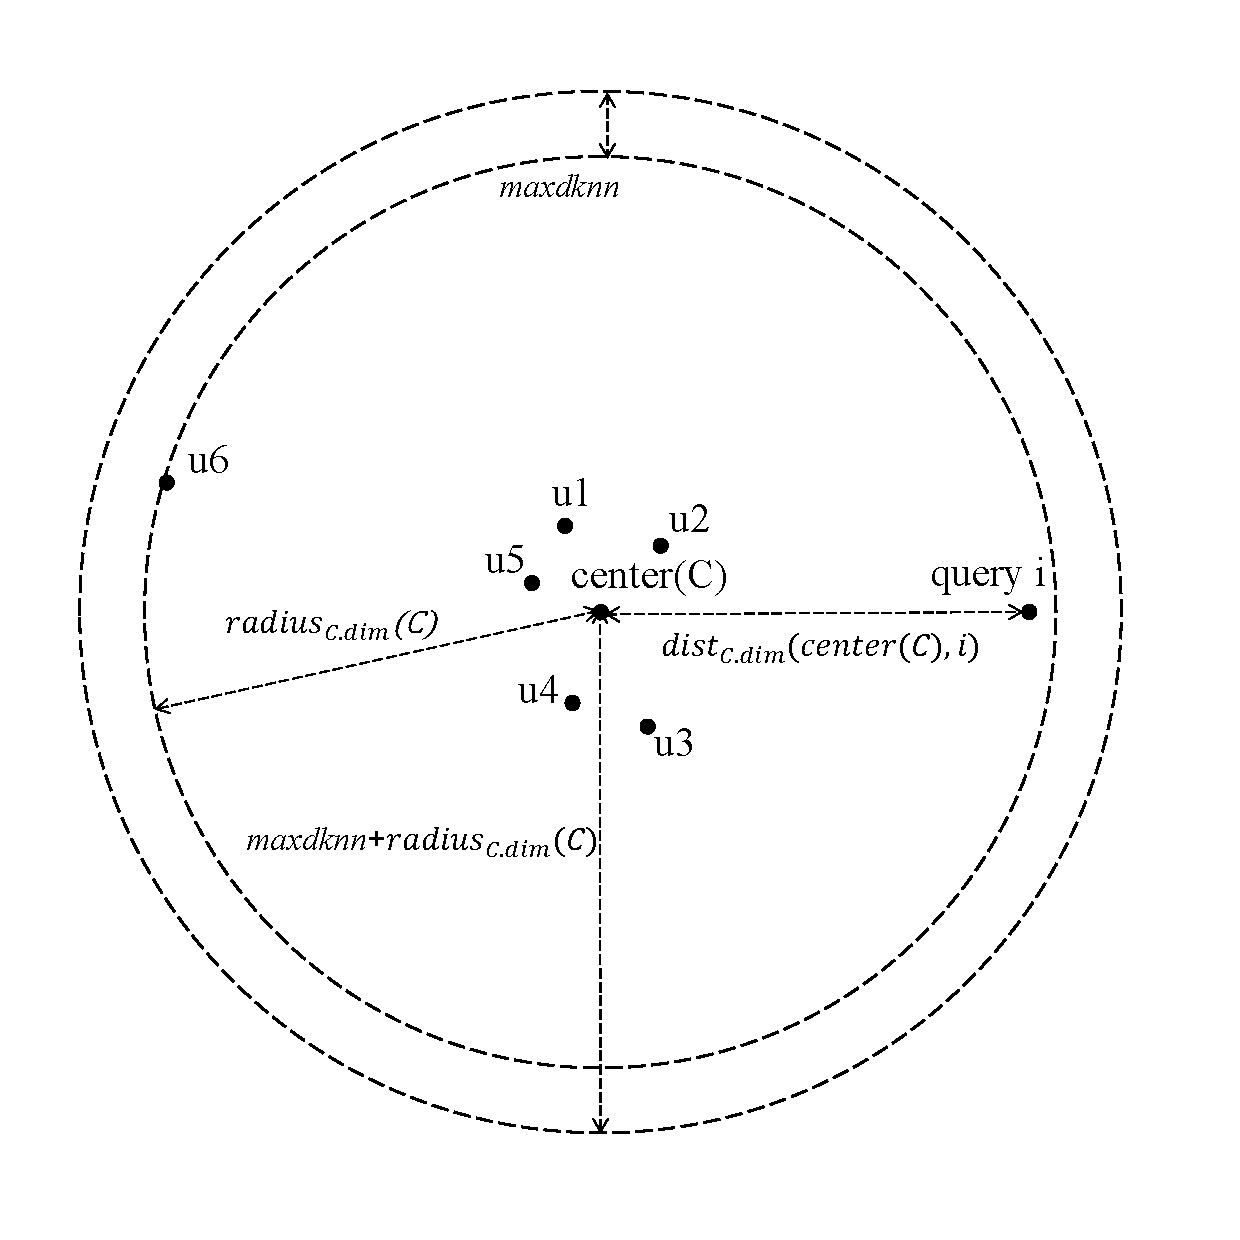
\includegraphics[width=0.5\textwidth]{Images/example_of_cluster_false.pdf}
    \caption{An example of Type  \uppercase\expandafter{\romannumeral2} error during the RKNN Search process on a HDR-Tree.}
    \label{fig:fdknnj-type_2_error_hdrtree}
\end{figure}

    As is shown in the Figure~\ref{fig:fdknnj-type_2_error_hdrtree}, it is obviously that all the points in the cluster C whose members are u1 to u6 on a HDR-Tree are not affected by the updated point i in \textit{i}, which is the query point of RKNN here. However, because distance between the point u6 in C on the back side of i and the center of C is too large, which makes the value  $radius_{C.dim}(C)$ in the pruning formulation large and enables the value $dist_{C.dim}(center(C), i) - radius_{C.dim}(C)$ on the left side of the pruning formulation to be smaller than the value of $maxdknn(C)$ on the right side of the pruning formulation, which guide the RKNN Search process into the sub-tree of C whose internal points are actually not affecetd by i.

    The second kind of cases is because of the loss of the distance information because of the distance calculation using the number of dimensions corresponding to the visited cluster C, which is smaller than the number of full dimensions. Lets consider a case where the difference between the distance from the center of the visited cluster C on the HDR-Tree to the query point i on full dimensions and the radius of C on full dimensions is not smaller than maxdknn, which can be written in mathematical language as $dist_{full dimensional}(center(C), i) - radius_{full dimensional}(C) \geq maxdknn(C)$. It is very obviously that in such case, all the points in C are impossible to be affected by i, and further RKNN Search implemented on the sub tree of C is unnecessary. However, even when $dist_{full dimensional}(center(C), i) - radius_{full dimensional}(C) \geq maxdknn(C)$, it is possible that we still have $dist_{C.dim}(center(C), i) - radius_{C.dim}(C)< maxdknn(C)$, which means the condition for further RKNN Search into the sub-tree of C holds and RKNN Search is guided into the sub-tree of a cluster whose internal points are not affected. This is because the decreasing effect of PCA on the Euclidean distance between different pairs of points can be different, which means that $dist_{full dimensional}(center(C), i) - dist_{C.dim}(center(C), i)$ might be smaller than $radius_{full dimensional}(C)- radius_{C.dim}(C)$, and lead to the value of $dist_{C.dim}(center(C), i) - radius_{C.dim}(C)$ to be smaller than  $dist_{full dimensional}(center(C), i) - radius_{full dimensional}(C)$, and be smaller than maxdknn. In the case introduced above, a cluster C on HDR-Tree whose internal points are not affected by i is considered to need to do further rknn into because of the distance information loss brought by PCA.   

Based on the deduction above, we can find that the distance analysis between the clusters on the HDR-Tree and the query points in \textit{i} for RKNN Search on low-dimensional space in order to recognize the clusters that need further RKNN Search into before the calculation of the full-dimensional distance between the points in the leafnodes of the HDR-Tree and the updated points in \textit{i} (also serve as query points) to finally find the affected points in \textit{U} can cause type  \uppercase\expandafter{\romannumeral2} error. And such type  \uppercase\expandafter{\romannumeral2} error will bring a number of distance calculation of full-dimensional between the points whose KNN lists are not affected and the updated points in \textit{i}. Such full-dimensional distance calculation might account for a considerable proportion of time cost in the whole RKNN Search process. Such type  \uppercase\expandafter{\romannumeral2} error can also happen in the KNN Search process on the Delta Tree \& HDR-Tree stucture and happen in the RKNN Search and KNN Search on the data structure of Delta Tree \& HDR Tree \& Clusters. 

As a result, in order to reduce the time cost of the full-dimensional distance calculation between the "unwanted points" (i.e., the points in the leafnodes of the HDR Tree which are not affected by the query points and the points in the leafnodes of the of the Delta Tree which are not the KNN members of the query points) brought by the type  \uppercase\expandafter{\romannumeral2} error and the query points, we proposed a new pruning method. In order to get rid of the error brought by analysis of the geometric relationship between clusters and clusters or points to clusters, this newly proposed method is based on geometric relationship analysis between points and points. This new pruning method uses the low-dimensional distance between the points as pruning bound to get rid of full-dimensional distance calculation to accelerate the whole process. Beside, we will provide the theoretical deduction of how to decide the optimal number of dimensions on which the low-dimensional distance serving as bound should be calculated. As is memtioned before, the method can be combined with the structure of Delta Tree \& HDR Tree or the structure of Delta Tree \& HDR Tree \& Clusters to accelerate the RKNN Search and the KNN Search within the calculation process of FDKNNJ. Below, we only introduce how to combine this pruning method with the HDR Tree within the Delta Tree \& HDR Tree structure to accelerate the RKNN Search process within the FDKNNJ process based on the Delta Tree \& HDR Tree structure. Application of this pruning method on other structures for KNN or RKNN Search is extremely similar to the situation we introduce below.

After being combined with the newly proposed pruning method, the algorithm for RKNN Search on a HDR Tree would be as the algorithm 4. 

\begin{algorithm}[t]
%\footnotesize
\caption{userSearch}\label{alg:user-search}
\begin{algorithmic}[1]
\Require node $node$, item $i$, mode $m$ 
\Ensure The affected user set $R_p$

\IF{$node$ is a $LN$}
    \FOR{each users $u_i$ in $node$}
      \IF{$dist_{d}(i,u_i)\leq u_i.dknn$}
          \IF{$dist(i,u_i)\leq u_i.dknn$}
              \STATE add $u_i$ in $R_p;$
          \ENDIF
      \ENDIF
    \ENDFOR
\ELSE
    \STATE $C_p = NLN.clusters;$
    \FOR{each clusters $C_j : C_p$}
		\IF{$dist_{ld}(center(LN), center(c_j)) - radius(c_j) - radius(LN) \geq maxbound$}
		  \STATE userSearch $(node.children[j],i,m);$
        \ENDIF
    \ENDFOR
\ENDIF
\end{algorithmic}
\end{algorithm}

What makes the algorithm different from that algorithm without our newly pruning method on a HDR  Tree is that on the 3-th line and on the 7-th line, we add a new IF structure to judge if the distance $dist_{d}(i,u_i)$ between the visited user $u_{i}$ in the leafnode and the query point $i$ is smaller than the dknn value of $u_i$. Only when such distance in low-dimensional space whose number of dimensions can be optimized theoretically is smaller than dknn of $u_i$ should we calculate the full dimensional distance $dist(i,u_i)$ between $u_i$ and $i$ and decide if $u_i$ is affected by $i$ according to the comparison of $dist(i,u_i)$ and the dknn value of $i$. By this method, we can accelerate the RKNN Search process by decreasing the number of full-dimensional distance calculation between the points in the leafnode of the HDR Tree which are not affected and the updated points in \textit{i} because some of the unaffected points are pruned by low-dimensional distance to the updated points in \textit{i}. However, such inserted pruning step can also bring additional calculation. For example, for an affected point, one additional time of low-dimensional distance calculation is brought, and for a point which is not affected but whose $dist_{d}(i,u_i)$ is smaller than its dknn value, one additional time of low-dimensional distance calculation is also brought. As a result, in order to make our pruning step effective and perform best, we need to theoretically analyze the relationship between the time cost of the total computation related to a leafnode in the HDR Tree and the value of d and attempt to find the optimal d. It is obviously that if we take a larger d, the proportion of points that need two times of distance calculation including one time of full-dimensional and one time of d-dimensional can be decreased because larger d is, $dist(i,u_i)-dist_{d}(i,u_i)$ will be smaller and $dist_{d}(i,u_i)$ is more possibly to be larger than the dknn of $u_i$. However, larger d can improve the time cost of the calculation of the low-dimensional distance between the points in the leafnodes and the updated points in \textit{i}. As a result, it is not a trivial work to find the optimal d that can provide the lowest time cost of the calculation within the leafnodes of the HDR Tree. Below we will build up a metric to estimate the expectation of the time cost of the calculation within the a leafnode in the HDR Tree during the RKNN Search of an arbirary query point. Based on the metric, we can find the relationship between the expectation of the time cost within one leafnode on the HDR Tree during the RKNN Search of a query point and the chosen value of d, so that we can find the optimal d that minimize the expected time cost. 

~\\
\textit{Preparation work of the cost model}

 We make an assumption that the time cost of one time of multiplication and the time cost of one time of addition and the time cost of one time of square root are the same and the time cost of each of the calculation above is regarded as 1. As a result, for the distance calculation between two points X and Y in d-dimensional space which is $\sqrt{\sum\limits_{i=1}\limits^{d}{(x_{i}-y_{i})^2}}$, its time cost is 4d. 
 
 For an arbitrary updated point $i$ in \textit{i} which is also a query for RKNN Search on the HDR Tree, we have the assumption below:
 
 1. For an arbitrary leafnode $LF$ visited during the RKNN Search process for $i$ on the HDR Tree, the expectation value of the number of points in $LF$ is $N$. It is obviously that $N$ is a value that is not affected by the choice of $d$, but only depend on the distribution of the dataset. 

 2. For an arbitrary point in $LF$, the possibility that it is affected by $i$ is $p_{1}$. It is obviously $p_{1}$ is a value that is not influenced by the choice of $d$, but only depend on the distribution of the dataset. We can use some sampling methods to gain $p_{1}$. For example, after calculating the KNNJoin result of \textit{u} and \textit{i} in the initial state and building up the HDR Tree and the Delta Tree of \textit{u} and \textit{i} in the initial state, we can add some points which are uniformly distributed among all the leafnodes of the Delta into \textit{i}. Then, we update the KNNJoin result of \textit{u} and \textit{i} by RKNN Search of such added points in \textit{i}. Through that RKNN Search process of such inserted points, we can obtain the statistic result of $p_{1}$.      

3. $v_{prune}$ is the the sum of the variance of the values of the data points in PCA space on the first $d$ dimensions on which we calculate the low-dimensional distance between the query points and the points in the leafnodes of the HDR Tree as pruning bounds. And $v_{sum}$ is the sum of the variance of the values of the data points in PCA space on all the dimensions. And $v=\frac{v_{prune}}{v_{sum}}$. It is obviously that $v$ is of positive relationship with $d$. Because of the feature of PCA, the increasing trend of $v$ would be very dramatic when $d$ is of low levels and tend to fatten out when $d$ increases to a high level.  Based on the observation before, we suppose that the relationship between $d$ and $v$ is $v=k_{1}ln(d)+b_{1}$, where $k_{1}>0$. $k_{1}$ can be gained by some sampling methods. For example, when calculating the PCA matrix of the dataset, we can gain $k_{1}$ by fitting the curve using the numbers of the front lines in the PCA matrix and the sums of the corresponding eigen values of the co-variance matrix of the original dataset.    

 4. For an arbitrary point that is not affected by $i$, the possibility that it takes two times of distance calculation including one time of full-dimensional and one time of $d$-dimensional to recognize that it not affected by $i$ is $p_2$. It is obviously that $p_2$ is affected by the value of $v$. When $v$ improves because $d$ improves, more distance information can be caught by the first $d$ dimensions in the PCA space on which we calculate the pruning distance. Therefore, $\frac{dist_{d}(i,u_i)}{dist(i,u_i)}$ will get larger. As a result, for a point $u_{i}$ in a leafnode on the HDR Tree which is not affected by the query point $i$, the possibility that $dist_{d}(i,u_i)<dknn$ gets smaller, so the possibility that it takes two times of distance calculation including one time of full-dimensional and one time of low-dimensional to recognize that $u_{i}$ is unaffected by the query point $i$ gets smaller. Model of the relationship between $p_{2}$ and $v$ can be various according to the distribution of the dataset. In this paper, we heuristically assume that $v$ and $p_{2}$ form a negative linear relationship, meaning that $p_{2}=k_{2}v+b_{2}$, where $k_{2}<0$. $k_{2}$ can be gained by some sampling methods. For example, we can add some points which are uniformly distributed among all the leafnodes of the Delta Tree into \textit{i}. Then, we update the KNNJoin result of \textit{u} and \textit{i} by RKNN Search of such added points in \textit{i} using different pruning dimensions which bring different corresponding values of $v$ and $p_{2}$, after which, we can fit the curve of $p_{2}$ and $v$ using the gained pairs of values of $v$ and $p_{2}$.

 5. We assume that the number of the full dimensions of the dataset is D.

 6. We use $T$ to represent the expectation of the amount of calculation within a leafnode on the HDR Tree when RKNN Search of a query point. 

 ~\\
\textit{Cost model of the calculation within a HDR leafnode}

Now we build up the estimation of the expectation of the calculation amount within a Leafnode $LF$ on the HDR Tree when RKNN Search of a query point $i$ with the number of pruning dimensions on the leafnodes of the HDR Tree as $d$, and try to find the value of d that minimizes that expectation of calculation amount. When the RKNN Search goes into a Leafnode of the HDR Tree, the main calculation will be the distance calculation. As a result, when estimating the expectation of the amount of calculations that happen within $LF$, we only take the calculation of distance into account. Based on the conditions given in the preparation work of the cost model, we can gain that:

~\\
$T=4N(p_{1}(d+D)+(1-p_{1})p_{2}(d+D)+(1-p_{1})(1-p_{2})d)$

$=4N(p_{1}D+D(1-p_{1})(k_{2}b_{1}+b{2})+D(1-p_{1})k_{1}k_{2}ln(d)+d)$

~\\
$\frac{\text{d}T}{\text{d}d}=D(1-p_{1})k_{1}k_{2}\cdot \frac{1}{d}+1$

~\\Then we let $\frac{\text{d}T}{\text{d}d}=0$, we can gain the equation that $D(1-p_{1})k_{1}k_{2}\cdot \frac{1}{d}+1=0$, after solving that equation, we can gain $d=-D(1-p_{1})k_{1}k_{2}$, and when $d<-D(1-p_{1})k_{1}k_{2}$, $\frac{\text{d}T}{\text{d}d}<0$, and when $d>-D(1-p_{1})k_{1}k_{2}$, $\frac{\text{d}T}{\text{d}d}>0$, As a result, we can gain that $d=-D(1-p_{1})k_{1}k_{2}$ is the optimal value to minimize the expectation of the calculation amount within $LF$ during the RKNN Search process of $i$ on the HDR Tree. 

In the discussion before, we propose a discovery that there might be considerable amount of points in the leafnodes of the HDR Tree that are not affected by the query point when RKNN Search of the query point goes into the leafnodes. This is because of the failure of pruning such unaffected points on the higher structure of the HDR Tree because of the \uppercase\expandafter{\romannumeral2} errors. Those \uppercase\expandafter{\romannumeral2} errors are brought from the analysis of the geometric relationship of low-dimensional on the non-leafnodes of the HDR Tree. Such unaffected points in the leafnodes of the HDR Tree can bring heavy calculation load if their distance of full-dimensional to the query point is calculated directly to be used for judging whether they are affected by the query point. We present a pruning method that can be used on the leafnodes of the HDR Tree when RKNN Search of a query point. This method can reduce the load of the calculation of full-dimensional between the query point and the points in the leafnode that are not affected by the query point by introducing a kind of pruning bounds that are the distance between the points in the leafnode and the query point on a specific number of dimensions. And we give out the method to theoretically confirm the optimal number of dimensions on which we calculate the low-dimensional distance as pruning bounds to minimize the expectation of the calculation amount on the leafnodes. Note that this method can also be combined with the Delta Tree \& HDR Tree structure and the $\Delta$-Tree \& HDR Tree \& Clusters to accelerate the process of KNN Search and the process of RKNN Search during the FDKNNJ process. And methods to confirm the optimal number of dimensions for pruning distance are very similar with the method used on the HDR Tree.%   
\end{comment}



\begin{comment}

The construction process of the Fully Dynamic Tree is undertaken in a top-down fashion. Initially, we use PCA to transform user data points into lower dimension points based on tree hierarchy. Furthermore, we also transform the item data points of the $\Delta$-tree to lower dimensions based on tree-level hierarchy. We set a fixed fanout value for the tree and apply the widely used k-means algorithm to partition the user set into clusters. If the number of users within a node falls below a predefined threshold $\theta$, we consider it a leaf node. Conversely, nodes with a higher number of users are classified as non-leaf nodes and are placed into a First-In-First-Out (FIFO) queue for further partitioning. This process continues until the queue is empty.

It is essential to note that it is not a height-balanced tree, but it is particularly efficient, as real-world datasets often exhibit skewness. Dense clusters are divided into finer-grained clusters to enhance pruning efficiency during the search process. We use the fanout value to estimate the height of the tree i.e., $L = [log_fN]$, where $f$ represents the fanout and $N$ denotes the number of user data points. The $\theta$ is set to a value that prevents the tree's actual height from deviating significantly from $L$. When the level of a cluster during construction exceeds $L$, and its size surpasses $\theta$, we continue partitioning the cluster using the full-dimensional user set, implying $d_l = d$ (if $l > L)$.

To enable the mapping of new items from the original space to the corresponding lower-dimensional spaces, we store the transformation matrix obtained during PCA. The HDR Tree encompasses users and their kNN, and the $\Delta$-tree includes all item sets; both are constructed using this identical procedure. The $\Delta$-tree is employed to determine the kNN for each user, enhancing pruning capabilities during the search process.


\subsection{Algorithms for Update Operations}
In our proposed approach, we address four distinct cases:

\begin{enumerate}[left=0pt, label=TYPE \arabic*:]
  \item Insertion of Users into HDR Tree
  \item Insertion of Items into $\Delta$-Tree
  \item Deletion of Items from $\Delta$-Tree
  \item Deletion of Users from HDR Tree
\end{enumerate}

In this section, we will elaborate on each case in detail. The HDR Tree encompasses all user data points and their respective $k$ nearest neighbor item sets, while the $\Delta$-Tree contains all item data points.

\subsubsection{Case 1: Insertion of Users}
%In a sequential insertion scenario, adding a user data point to the HDR Tree requires finding the $k$ nearest neighbors for that user, updating the user's $dknn$ value, and updating the $maxdknn$ value for the affected cluster. Unfortunately, this approach is quite time-consuming and less efficient when inserting multiple users simultaneously. To address this challenge, we propose batch insertion of users for FdkNNJ Tree.

%In the process of inserting a new user, it is crucial to assign them to appropriate user clusters efficiently. While inserting, we must identify its $k$ closest neighbor items and include them in the user's recommendation list $R_l$ (i.e., the user's kNN list). 
%
%During user allocation, our goal is to minimise the computational overhead by reducing the number of distance computations. To achieve this, we calculate distances between users and the centers of clusters, which are transformed into reduced dimensionality.
%

%When dealing with a large volume of new users, it is highly probable that each cluster will accommodate numerous new users. In such scenarios, instead of handling users one at a time (i.e., computing kNN for each newly added user individually), we propose a more streamlined approach: batch updates. In this method, clusters that consist of the newly inserted users operate as batches, and we process one batch at a time. Let's consider the scenario of updating only one or a few users. We need to find the $k$ nearest neighbors for that user, update the user's $dknn$ value, and update the $maxdknn$ value for the affected cluster. So, updating one-by-one users turns out to be quite time-consuming and less efficient when we have to insert multiple users simultaneously. Thus, we focus on the batch update approach for newly added users.
%

In our proposed approach, aside from the HDR tree on the user side, we introduced an additional structure that is composed of several user clusters. Here, the number of clusters can be determined by users, and any clustering approach can be used. In our work, we used the k-means clustering. Initially, the entire user set is clustered to form these user clusters, creating a user structure distinct from the HDR Tree.

Upon inserting a batch of users, we need to compute the kNN and insert users into the HDR Tree. Subsequently, we also add users to the user cluster structure formed during the initial clustering process. Each user cluster's center is defined by the initial user set and is then surrounded by the newly inserted users. This differs from prior approaches where leaf nodes were surrounded by newly inserted users. Assigning users to clusters rather than individual leaf nodes becomes crucial as it addresses potential scalability issues when dealing with a large number of users.




We begin by traversing through the root level of the $\Delta$-tree. In the case of single-user insertion, this pruning technique is used to reduce the search space:

$dist_{node.dim}(u_i, c_j) - radius(c_j) \geq bound$

Here, depending on the node level of the $\Delta$-Tree, we calculate the distance between the user and the cluster center in lower dimensions using PCA. The bound serves as a pruning parameter to decide whether to explore that non-leaf node or prune it. Specifically, the bound is defined as $dknn$, which is:

$bound = dist (u,$ farthest item in user's kNN list)

As discussed in \cite{ukey2023efficient}, the distance between the user and the cluster center in the full dimension is always greater than or equal to the distance in lower dimensions. Therefore, before entering a non-leaf node in the HDR Tree, we transform the user to lower dimensions using a precomputed transformation matrix. To clarify the condition further, it is expressed as follows:

$dist(u_i, i_j) \geq dist_{node.dim}(u_i, i_j) \geq dist_{node.dim}(u_i,c_j) -\\
radius(c_j) \geq bound$

\end{comment}

\begin{comment}
for batch insertion, we employ the following pruning technique:

$dist_{node.dim}(center(LN), c_j) - radius(c_j) - radius(LN) \geq maxbound$

In this case, there is no need to calculate distances or values since we have already stored the radii for all clusters and leaf nodes, as well as the $maxdknn$ values. Similarly, when constructing the index structure for the fully dynamic tree, we also stored the distance from the leaf node of HDR Tree to the cluster center of the $\Delta$-Tree.
This novel pruning method significantly enhances the efficiency of finding the kNN for each new user across the $\Delta$-Tree.

\end{comment}

\begin{comment}
By adopting batch updates, we can significantly optimise the insertion process. This approach minimises the computational load by efficiently grouping users into clusters. However, it is important to note that if a cluster contains only a few users, we process them individually.

In the presented fully dynamic kNN join structure illustrated in Figure~\ref{fig:fdknnj-user-insertion}, we insert the set of users. Initially, we extracted user $u_{20}$ from the user input stream and added it to the HDR Tree. This process involves evaluating pruning conditions and placing the user within the relevant clusters and non-leaf nodes. We also need to find the $k$ nearest neighbors for the newly added user. In our scenario, considering $k$ = 5, our objective is to determine the 5 closest neighbors for $u_{20}$.



Unlike traditional exhaustive search (i.e., using a sliding window), our proposed approach involves employing the $\Delta$-tree for this purpose. We initiate the search from the root node of the $\Delta$-tree and progress towards the LN, which contains the closest neighbors. Through the implementation of strong pruning techniques, we avoid the need to inspect every single cluster. Our pruning method helps to skip clusters that do not yield promising solutions, significantly enhancing the efficiency of the process. During the insertion of a new user, our focus lies in updating the kNN list and dknn value of the users. After batch insertion, we update the maxdknn value of the HDR Tree, which significantly reduces computational overhead.

The Algorithm \ref{alg:update_users}, updates a data structure called a Fully Dynamic Tree with newly added user data points. The tree is organised into different nodes, including leaf nodes and non-leaf nodes.

\begin{algorithm}[t]
\caption{updateUser (node, U)}\label{alg:update_users}
\begin{algorithmic}[1]
\Require Node object 'node', User object 'U'
\Ensure Update the HDR Tree with a new user
\IF{$node == LN$}
    \STATE $maxL \gets 0$
    \IF{$LN.cluster.number < \theta$}
        \STATE $U.computeKNN()$
        \STATE $LN.cluster.Users.append((U.dknn, U))$
    \ELSE
        \STATE $ maxL \gets max(maxL, level)$
        \STATE $updateConstruct(node);$
    \ENDIF
\ELSE
    \STATE $Cp \gets NLN.clusters$
    \STATE $minDist \gets MAX\_FLOAT$
	\STATE $clust \gets 0$
    \FOR{$j$ in $range(0, Cp.size())$}
        \STATE $d \gets dist(U, Cp[j])$
		\IF{$d < minDist$}
            \STATE $minDist \gets d$
            \STATE $clust \gets j$
        \ENDIF
    \ENDFOR
    \IF{$Cp[clust].radius < minDist$}
        \STATE $Cp[clust].radius \gets minDist$
    \ENDIF
    \STATE $parent \gets NLN$
    \STATE $updateUser(NLN.children[clust], U)$
\ENDIF
\end{algorithmic}
\end{algorithm}

\begin{algorithm}
\caption{updateConstruct(node)} \label{alg:update_construct}
\begin{algorithmic}[1]
\Require Node object `node' FOR tree construction
\Ensure Adapt the HDR-Tree structure
    \STATE $q \gets empty Queue$
    \STATE $q.push(node)$
    \STATE $maxL \gets 0$
    \WHILE{not $q.empty()$}
        \STATE $node \gets q.front()$
        \STATE $q.pop()$
        \STATE $C_p \gets node.clusters$
        \FOR{$C_j$ in $C_p$}
            \IF{$C_j.number < \theta$}
                \STATE $LN \gets new LeafNode(C_j)$
                \STATE $node.children.append(LN)$
                \STATE $C_j.ptr \gets LN$
            \ELSE
                \STATE $level \gets node.l + 1$
                \STATE $maxL \gets max(maxL, level)$
                \STATE $C_{pp} \gets new Clusters(C_j, 4, data.T[level - 1])$
                \FOR{$C_j in C_{pp}$}
                    \IF{$C_j.Users.size() > 0$}
                        \STATE $C_j.maxdknn \gets C_j.Users[0].dknn$
                        \FOR{$t$ in $C_j.Users$}
                            \STATE $C_j.maxdknn \gets max(C_j.maxdknn, t.dknn)$
                        \ENDFOR
                    \ENDIF
                \ENDFOR
                \STATE $C_j.l \gets level$
                \STATE $NLN \gets new NonLeafNode(C_{pp}, level)$
                \STATE $node.children.append(NLN)$
                \STATE $C_j.ptr \gets NLN$
                \STATE $q.push(NLN)$
            \ENDIF
        \ENDFOR
    \ENDWHILE
\end{algorithmic}
\end{algorithm}

Basically, it is responsible for updating the tree with a new user, represented by the $U$. It starts by checking the type of the current node it is examining (line 1). If the node is a leaf node, it checks if the number of users in the leaf node's cluster is less than some threshold ($\theta$). If so, it computes the $k$ nearest neighbors of the user $U$ over $\Delta$-tree and adds this user to the cluster (lines 3-5).

If the number of users in the leaf node's cluster exceeds the $\theta$, it proceeds to the $\textit{updateConstruct()}$ function, which is responsible for constructing new levels of the tree. It essentially splits the current node into multiple child nodes (both leaf and non-leaf) to accommodate more users (lines 6-8).

In the $updateConstruct()$ function, a breadth-first search (BFS) approach is used to traverse the tree and construct new nodes as needed. If a cluster in a non-leaf node exceeds the threshold, it creates a new non-leaf node and possibly more leaf nodes beneath it to distribute the users further in the hierarchy. The algorithm also updates the levels and pointers accordingly.

On the other hand, if the current node is a non-leaf node, the algorithm calculates the distance between the new user and the clusters within the non-leaf nodes. The user is then assigned to the closest cluster ( i.e., the cluster with the minimum distance) (lines 9-17). The $radius$ of the selected cluster is updated if the user is farther away than the existing $radius$ (lines 18-19). The function then recursively calls itself on the child node corresponding to the selected cluster (line 21).

This algorithm maintains a hierarchical structure to efficiently organise users into clusters while ensuring that no cluster exceeds a certain size threshold. As new users are added, the tree dynamically adjusts its structure to maintain this balance.



\subsubsection{Case 2: Batch Insertion of Items}\label{subsubsec:insertion-items}
In the context of item updates, which include both insertions and deletions, we perform these operations on both the $\Delta$-tree and the HDR Tree. Our procedure begins with the insertion of an item data point into the $\Delta$-tree, followed by the update of the leaf node. To insert an item into the appropriate leaf node, we traverse the tree. Within each leaf node, we check whether the number of items exceeds a predefined threshold. If this $\theta$ is exceeded, we must further split the node.

for each item data point insertion, we must identify the set of affected users, all of whom require updates. Fortunately, the insertion process is not computationally intensive. 

\begin{example}
    for instance, when inserting an item, say, $i_{11}$, which affects users $\{u_3, u_{84}, u_9\}$. We are considering that each user already has a list of $k$ items in their recommendation list. Adding $i_{11}$ to this list increases the count to $k+1$ items. Consequently, we can simply remove the $k$-th element from the list. This approach is justified because the new item is undoubtedly closer to the user than the $k$-th element. As a result, the insertion operation affects users $\{u_3, u_{84}, u_9\}$. In this manner, we avoid recomputing the kNN for affected users from scratch and eliminate the need to search within the $\Delta$-tree.
\end{example}

Previously, to identify affected users for each operation, we used the following pruning condition:

$dist_{node.dim}(i_j, c_j) - radius(c_j)\geq maxdknn$

for batch updates, we have enhanced our pruning technique as follows:

$dist_{node.dim}(center(LN), c_j) - radius(c_j) - radius(LN) \geq maxdknn$

In this context, the center of the leaf node corresponds to the center of the $\Delta$-tree leaf node, while the center of the cluster corresponds to the HDR Tree cluster center. When this criterion is met, it results in the pruning of clusters.
These improvements optimise the efficiency of item insertions and deletions in both trees, significantly enhancing the overall performance of our approach.

\begin{algorithm}[t]
%\footnotesize
\caption{userSearch}\label{alg:user-search}
\begin{algorithmic}[1]
\Require node $node$, item $i$, mode $m$ 
\Ensure The affected user set $R_p$

\IF{$node$ is a $LN$}
    \FOR{each users $u_i$ in $node$}
        \IF{$dist(i,u_i)\leq u_i.dknn$}
            \STATE add $u_i$ in $R_p;$
        \ENDIF
    \ENDFOR
\ELSE
    \STATE $C_p = NLN.clusters;$
    \FOR{each clusters $C_j : C_p$}
		\IF{$dist_{ld}(center(LN), center(c_j)) - radius(c_j) - radius(LN) \geq maxbound$}
		  \STATE userSearch $(node.children[j],i,m);$
        \ENDIF
    \ENDFOR
\ENDIF
\end{algorithmic}
\end{algorithm}

The Algorithm \ref{alg:user-search} is used to identify affected users by item update operation based on certain pruning conditions. The algorithm takes the three main inputs: the current node ($node$), an updated (i.e., newly inserted or deleted) item ($i$), and a mode ($m$), which is item insertion or deletion. 
Initially, it checks whether the current node is a leaf node ($LN$) or not. In the case of a leaf node, representing individual users, the algorithm iterates through each user ($u_i$) within the $node$. For every user, it evaluates the distance between the given item $i$ and the user $u_i$. If this distance falls within the user's designated threshold $u_i.dknn$, indicating proximity, the user is added to the affected user set $R_p$ (lines 1-6).

When the current node is a non-leaf node ($NLN$), the algorithm proceeds differently. It obtains the clusters $C_p$ from the non-leaf node and iterates through each cluster $C_j$ within $C_p$. For each cluster, the algorithm calculates the distance between the center of the current $LN$ of $\Delta$-tree and the cluster center $C_j$ of HDR Tree. It then subtracts the radius of cluster $C_j$ and the radius of leaf node $LN$ from this distance. If this result is greater than or equal to a predefined maximum bound $maxdknn$, the algorithm recursively calls the $userSearch$ algorithm on the child node $node.children[j]$ (i.e., explore the child node). This algorithm recursively explores the tree structure to locate additional affected users based on spatial relationships (lines 7-14).

\subsubsection{Batch Deletion of Items}\label{subsubsec:deletion-items}

Case~\ref{subsubsec:deletion-items} shares similarities with Case~\ref{subsubsec:insertion-items} but with a crucial distinction when it comes to item deletion. In this scenario, we must identify the affected users, but the update operation for their kNN lists is considerably more computationally demanding. 

\begin{example}
    To illustrate, consider the deletion of an item, say, $i_{11}$, which impacts users $u_3, u_84, u_9$. As a matter of practice, each user maintains a recommendation list containing k items. Removing $i_{11}$ from these lists reduces the count to k-1 items. To determine the appropriate kth element, we must search for the k-th closest item within the Delta Tree.
\end{example}

We initiate this process from the root of the tree and apply a similar pruning strategy as employed during item insertion. This allows us to prune away unnecessary clusters, ultimately leading us to the appropriate $k$-th element within the leaf node of the Delta Tree. In essence, we update the kNN lists and the $dknn$ values as well. We then update all affected clusters resulting from the batch deletion. This approach helps reduce the computational power and time required to compute, which makes our approach more efficient.

Basically, Case \ref{subsubsec:d
eletion-items} addresses the batch deletion of items from the $\Delta$-tree, with a focus on the efficient update of kNN lists for affected users from the HDR Tree, enhancing the overall performance of our approach.


\subsubsection{Batch Deletion of Users}\label{subsubsec:deletion-users}
Case 4 is a straightforward approach where you do not need to perform any costly operation after the deletion of users from the HDR Tree. Thus, we will refrain from delving into further details of this case.

\begin{example}
    To illustrate, consider the scenario where we wish to remove a user from the HDR Tree. In this context, the process involves removing the user from all non-leaf nodes and the leaf node containing the user data point. We do not need to find affected users or calculate kNN for them, which is a costly operation.
\end{example}

It is important to note that if the deleted user occupies the outermost position within the cluster, then we need to update to the $maxdknn$ value of the cluster. Moreover, if the deleted user was the sole occupant of the leaf node, it becomes feasible to remove the entire leaf node altogether. This procedure efficiently removes users without complex operations, making it practical in the HDR Tree framework.



\end{comment}

\begin{comment}
For the data partitioning process, we use the clustering method. Various clustering metods are available, and in this paper, we use the k-means method. At the root level, the vectors in $U$ are clustered into a lower-dimensional space, referred to as $d_1$, using PCA. Subsequently, this transformed data is partitioned into $f$ clusters, denoted as $C_1, C_2,\ldots, C_f$ if the fanout value is $f$. Moving to the second level, each cluster $C_i$ from the previous level is further subdivided into sub-clusters, denoted as $C_{i1}, C_{i2},\ldots, C_{if}$, within a $d_2$-dimensional space. This hierarchical partitioning continues for every subcluster at each level $l$ of the tree, where clusters are partitioned in a $d_l$-dimensional space. The original users, at their full dimensionality, are stored in the leaf nodes of the tree.

Each non-leaf node is represented by a tuple of attributes for each of its clusters. These attributes include the cluster's center ($c_i$) in the $dl$-dimensional space, its radius ($r_i$), the number of users ($num$) it contains, the maximum distance ($maxdknn$) between the users in the cluster and their $k$ nearest neighbor items, the level ($l$) at which the cluster resides, and a pointer ($ptr$) to the next hierarchical level node. In contrast, leaf nodes store the actual user set $U_j$ within the cluster without any dimensionality reduction.
The index structure is created for both the user and item trees using a combination of user tree and item tree index structures, leveraging hierarchical partitioning and PCA-based dimensionality reduction to efficiently organise and access the data.

\end{comment}


\begin{comment}
    \item  $M$ lists of probability distributions, where the $i$-th list contains $B_i$ probability distributions denoted by $F_{ij}$ for $1 \leq i \leq M,\, 1 \leq j \leq B_i$, with $F_{ij}$ representing the $j$-th distribution in the $i$-th list.
\end{comment}


\begin{comment}
Note that in computing the random variable $dist^{2}(q_{\mathcal{O}_i},v^{j}_{q_{\mathcal{O}_{i}}})/b_{p}^{2}$, $q_{\mathcal{O}_i}$ is treated as a fixed data point once it has been arbitrarily chosen from $\mathcal{O}_i$.
\end{comment}